\documentclass[12pt,italian]{article}
\usepackage[T1]{fontenc}
\usepackage{babel}
\usepackage[utf8]{inputenc}
\usepackage{enumitem}
\usepackage{subfiles}
\usepackage{multirow}
\usepackage{color}
\usepackage{titlesec}
\usepackage{longtable}
\usepackage{xcolor,colortbl}
\usepackage[hidelinks]{hyperref}
\usepackage{graphicx}
\usepackage{amsmath}
\usepackage{mdframed}
\usepackage{listings}
\usepackage{minted}
\usepackage{subfigure}

\usepackage[a4paper,width=180mm,top=25mm,bottom=25mm]{geometry}
\usepackage{afterpage}
\usepackage{array,ragged2e}
\usepackage{booktabs}

\graphicspath{{./immagini/}}

\definecolor{LightGray}{gray}{0.9}

\definecolor{codegreen}{rgb}{0,0.6,0}
\definecolor{codegray}{rgb}{0.5,0.5,0.5}
\definecolor{codepurple}{rgb}{0.58,0,0.82}
\definecolor{backcolour}{rgb}{0.95,0.95,0.92}

\newcolumntype{P}[1]{>{\RaggedRight\arraybackslash}p{#1}}
\newlist{tabitem}{itemize}{1}
\setlist[tabitem]{nosep,
                  topsep     = 0pt,
                  partopsep  = 0pt,
                  leftmargin = *,
                  label      = \textbullet,
                  before = \vspace{-1\baselineskip},
                  after = \vspace{-0.5\baselineskip}}

\hypersetup{
    linktoc=all,
    pdfpagemode=FullScreen,
}
\definecolor{Gray}{gray}{0.85}
\definecolor{LightCyan}{rgb}{0.88,1,1}
\title{WYD}
\author{
Giacomo Romanini 00874849\\
}
\date{Marzo 2025}

\begin{document}
\maketitle
\pagenumbering{gobble}
\newpage
\pagenumbering{gobble}
\tableofcontents
%%%%%%%%%%% Moduli per ogni sezione %%%%%%%%%%%%%%%

%\section{Abstract}

Wyd è un'applicazione che permette ai clienti di organizzare i propri impegni, siano essi confermati oppure proposti.\newline
Mette a disposizione due calendari, il primo con gli eventi in cui l'utente è convinto di partecipare, 
il secondo in cui vengono riuniti gli eventi a cui l'utente è stato invitato ma senza aver ancora dato conferma.\newline
L'utente ha la possibilità di creare, modificare, confermare o disdire un evento, ma anche condividerlo con altri o allegarci foto.
La condivisione di un evento può avvenire con applicazioni esterne tramite la generazione di un link o grazie all'ausilio di gruppi di profili.
Inoltre, al termine di un evento, l'applicazione carica automaticamente le foto scattate durante l'evento, per allegarle a seguito della conferma dell'utente.\newline  
L'utente può infatti cercare altri profili e creare gruppi con i profili trovati.\newline
Tutta l'interazione avviene tramite l'utilizzo di profili, che permettono di suddividere semanticamente gli eventi e le relazioni.\newline
\newpage
%\section{Abstract e Requisiti}

\subsection{Il progetto}

L'idea per il progetto di questa tesi nasce come risposta a un problema sempre più attuale in un mondo sempre più connesso.
La molteplicità di contatti, la velocità delle comunicazioni e l'accesso universale alle notizie 
rendono la creazione, l'organizzazione e la partecipazione ad eventi estremamente semplice ma al contempo frenetico.
Si fa fatica a seguire a tutte le occasioni a cui potremmo prendere parte.
Pensiamo alle riunioni di lavoro, alle serate tra amici, agli appuntamenti per un caffè.
Ma anche a una fiera, una convention aziendale, ad un concerto, alla partita di calcio o alla mostra dell'artista che ci è sempre piaciuto e che passa per una volta nella città vicina.
Queste occasioni spesso si accavallano o si finisce per dimenticarsene, potenzialmente creando delusione e/o frustrazione.\\
\\
Quando condividiamo un evento, a volte siamo noi a proporre, altre volte ci invitano. \\
Quando ci invitano, spesso magari abbiamo già un altro impegno, o magari un invito di un altro contatto a cui dobbiamo ancora dare conferma. 
E sul momento magari non ci si ricorda, si conferma per poi dover, purtroppo, disdire l'evento sovrapposto.\\
Quando invece siamo noi a proporre, potremmo trovarci nella difficoltà di trovare un evento da proporre, 
scrutando centinaia di profili social di tutti i locali di cui abbiamo sentito parlare nella speranza che propongano qualcosa, 
oppure non sappiamo se l'altra persona possa essere libera o meno. 
Questo problema si ripresenta ancora più grave nell'organizzazione di gruppo, in cui bisogna riuscire a far combaciare gli impegni di tre, quattro o più persone.\\
\\
Ecco quindi l'opportunità di creare uno strumento che permetta di semplificare la proposta e la gestione degli eventi, 
separando la proposta dalla conferma, per dare modo di valutare l'effettiva disponibilità ma anche rendere più facile un'invito a partecipare.
Allo stesso modo si può semplificare la ricerca di occasioni, creando uno spazio unico virtuale in cui pubblicare e consultare gli eventi.\\
\\
Alla base della funzionalità sussiste l'idea di affiancare alla classica agenda degli impegni presi (e quindi confermati) 
un'altro calendario in cui sono presenti tutti gli eventi a cui si potrebbe partecipare. 
La conferma di un evento lo sposterà all'interno dell'agenda.\\
Gli eventi creati potranno essere condivisi a persone o gruppi di persone, e sarà possibile vedere chi conferma la sua presenza.\\
Inoltre, nell'epoca delle immagini e della condivisione, si prevede la possibilità di condividere le proprie foto con chiunque abbia partecipato all'evento.\\
\\
La realizzazione di questo tipo di programma prevede particolarità che incrociano tante necessità diverse.
In primis la persistenza dell'agenda dell'utente, che deve essere mantenuta e aggiornata per garantire affidabilità e coerenza per un uso distribuito del servizio.
Si aggiunge poi l'aspetto della condivisione degli eventi, che vede necessario l'aggiornare tutti gli attori interessati dalle modifiche apportate.
Infine, il caricamento e salvataggio delle foto introduce la gestione di richieste e di memoria di dimensioni importanti.\\
\\
\clearpage

\subsection{Abstract del progetto}

Wyd è un'applicazione che permette ai clienti di organizzare i propri impegni, siano essi confermati oppure proposti.\newline
Mette a disposizione due calendari, il primo con gli eventi in cui l'utente è convinto di partecipare, 
il secondo in cui vengono riuniti gli eventi a cui l'utente è stato invitato ma senza aver ancora dato conferma.\newline
L'utente ha la possibilità di creare, modificare, confermare o disdire un evento, ma anche condividerlo con altri o allegarci foto.
La condivisione di un evento può avvenire con applicazioni esterne tramite la generazione di un link o grazie all'ausilio di gruppi di profili.
Inoltre, al termine di un evento, l'applicazione carica automaticamente le foto scattate durante l'evento, per allegarle a seguito della conferma dell'utente.\newline  
L'utente può infatti cercare altri profili e creare gruppi con i profili trovati.\newline
Tutta l'interazione avviene tramite l'utilizzo di profili, che permettono di suddividere semanticamente gli eventi e le relazioni.\newline

\newpage

\subsection{Raccolta dei requisiti}

\begin{itemize}
  \item[-] Per interagire con l’applicazione è necessario avere un utente registrato.
  \item[-] Per registrarsi l’utente deve inserire una mail univoca, e una password lunga almeno 6 caratteri.
  \item[-] L’utente ha a disposizione un’agenda con gli eventi confermati e una con gli eventi proposti.
  \item[-] L’utente può creare un evento, definendo, al minimo, la data di inizio e di fine.
  \item[-] La data di fine deve essere successiva alla data di inizio.
  \item[-] L’utente può modificare un evento.
  \item[-] L’utente può confermare un evento condiviso, o disdire un evento confermato.
  \item[-] L’utente può condividere l’evento ad altri profili tramite link o condividendo a un gruppo o ad altri profili singoli.
  \item[-] L’utente può caricare le foto relative ad un evento, con visibilità condivisa.
  \item[-] Alla scadenza dell’evento, se su dispositivo mobile, l’applicazione controlla le foto scattate durante l’evento. Se ce ne sono, l’utente verrà notificato e potrà eliminare o confermare le foto, che verranno quindi caricate.
  \item[-] L’utente può cercare altri profili e creare un’associazione tra il profilo cercato e quello che sta usando.
  \item[-] I profili possono avere associazioni tra loro, a coppie o come gruppi.
  \item[-] L’utente può avere più profili, vedere in contemporanea gli eventi di tutti i profili associati ma effettuare le azioni a nome di uno solo.
  \item[-] La conferma/disdetta, il caricamento delle foto e la modifica di un evento deve avvenire in tempo reale se i profili condivisi sono online, altrimenti ricevono gli aggiornamenti all’avvio dell’applicazione.
  \item[-] L'applicazione deve essere intuitiva e con brevi tempi di risposta.
  \item[-] L'applicazione deve poter funzionare con un elevato numero di richieste concorrenti.
\end{itemize}


\subsection{Tabella dei Requisiti}

\begin{tabular} {|P{1.3cm}|P{11.2cm}|P{3cm}|}
  \hline
  \textbf{ID} & \textbf{Requisiti}                                                          & \textbf{Tipo}  \\
  \hline
  R1F         & Registrazione di un account tramite l’interfaccia web                       & Funzionale     \\
  \hline
  R2F         & Identificazione attraverso mail univoca e password di almeno 6 caratteri    & Funzionale     \\
  \hline
  R3F         & Visualizzazione degli eventi confermati                                     & Funzionale     \\
  \hline
  R4F         & Visualizzazione degli eventi proposti                                       & Funzionale     \\
  \hline
  R5F         & Creazione di un evento impostando almeno la data di inizio e quella di fine & Funzionale     \\
  \hline
  R6F         & La data di fine deve essere successiva alla data di inizio                  & Funzionale     \\
  \hline
  R7F         & Modifica di un evento                                                       & Funzionale     \\
  \hline
  R8F         & La conferma di un evento lo sposta negli eventi confermati                  & Funzionale     \\
  \hline
  R9F         & La disdetta di un evento lo sposta negli eventi proposti                    & Funzionale     \\
  \hline
  R10F        & Caricamento delle foto di un evento                                         & Funzionale     \\
  \hline
  R11F        & Condivisione tramite link                                                   & Funzionale     \\
  \hline
  R12F        & Condivisione tramite gruppo o ad altri profili                              & Funzionale     \\
  \hline
  R13F        & Ricerca automatica delle foto sul dispositivo mobile                        & Funzionale     \\
  \hline
  R14F        & Conferma delle foto                                                         & Funzionale     \\
  \hline
  R15F        & Ricerca di altri profili                                                    & Funzionale     \\
  \hline
  R16F        & Creazione di un gruppo da due o più profili                                 & Funzionale     \\
  \hline
  R17F        & Visualizzazione dei profili collegati                                       & Funzionale     \\
  \hline
  R18F        & Creazione di un nuovo profilo                                               & Funzionale     \\
  \hline
  R19F        & Cambio del profilo attualmente in uso                                       & Funzionale     \\
  \hline
  R20F        & Aggiornamento in tempo reale delle modifiche agli eventi                    & Funzionale     \\
  \hline
  R1NF        & Per interagire l’utente deve essere autenticato                             & Non Funzionale \\
  \hline
  R2NF        & Velocità di richiesta iniziale dei dati                                     & Non Funzionale \\
  \hline
  R3NF        & Semplicità e fluidità dell'interfaccia grafica                              & Non Funzionale \\
  \hline
  R4NF        & Velocità in lettura e scrittura dei dati                                    & Non Funzionale \\
  \hline
  R5NF        & Velocità nella ricerca dei profili                                          & Non Funzionale \\
  \hline
  R6NF        & Scalabilità delle richieste                                                 & Non Funzionale \\
  \hline
\end{tabular}
\clearpage

\subsection{Analisi dei Requisiti}
\subsubsection{Vocabolario}

\begin{tabular} {|P{3.5cm}|P{9cm}|P{3cm}|}
  \hline
  \textbf{Voce}     & \textbf{Definizione}                                                             & \textbf{Sinonimi}                 \\
  \hline
  Account           & combinazione di mail e password che identifica un utente                         &                                   \\
  \hline
  Utente            & Persona che utilizza l’applicazione                                              &                                   \\
  \hline
  Profilo           & Entità logica che raggruppa eventi e interazioni                                 &                                   \\
  \hline
  Profili collegati & Profili a cui l'utente può avere accesso                                         &                                   \\
  \hline
  Gruppo            & Insieme di profili                                                               &                                   \\
  \hline
  Evento            & Azione(o previsione di azione) con una durata nel tempo                          &                                   \\
  \hline
  Data e ora evento & Indicazione temporale del momento in cui avverrà l'azione                        &                                   \\
  \hline
  Evento confermato & Evento a cui il profilo ha dato conferma di partecipazione                       &                                   \\
  \hline
  Evento proposto   & Evento a cui il profilo non ha dato conferma di partecipazione                   & Evento disdetto, evento condiviso \\
  \hline
  Email             & Indirizzo di posta elettronica del cliente utilizzata anche per l'autenticazione &                                   \\
  \hline
  Password          & Codice alfanumerico di almeno 8 caratteri                                        &                                   \\
  \hline
  Credenziali       & Insieme composto da email e password necessari per accedere al sistema           &                                   \\
  \hline
\end{tabular}



\subsubsection{Sistemi esterni}
\label{sec:esterno}

Il sistema non dovrà interfacciarsi con sistemi esterni.


\newpage %optional
\subsubsection{Casi d'uso}

\begin{figure}[h!]
  \centering
    \adjustbox{valign=c, width=0.9\textheight, angle=90}{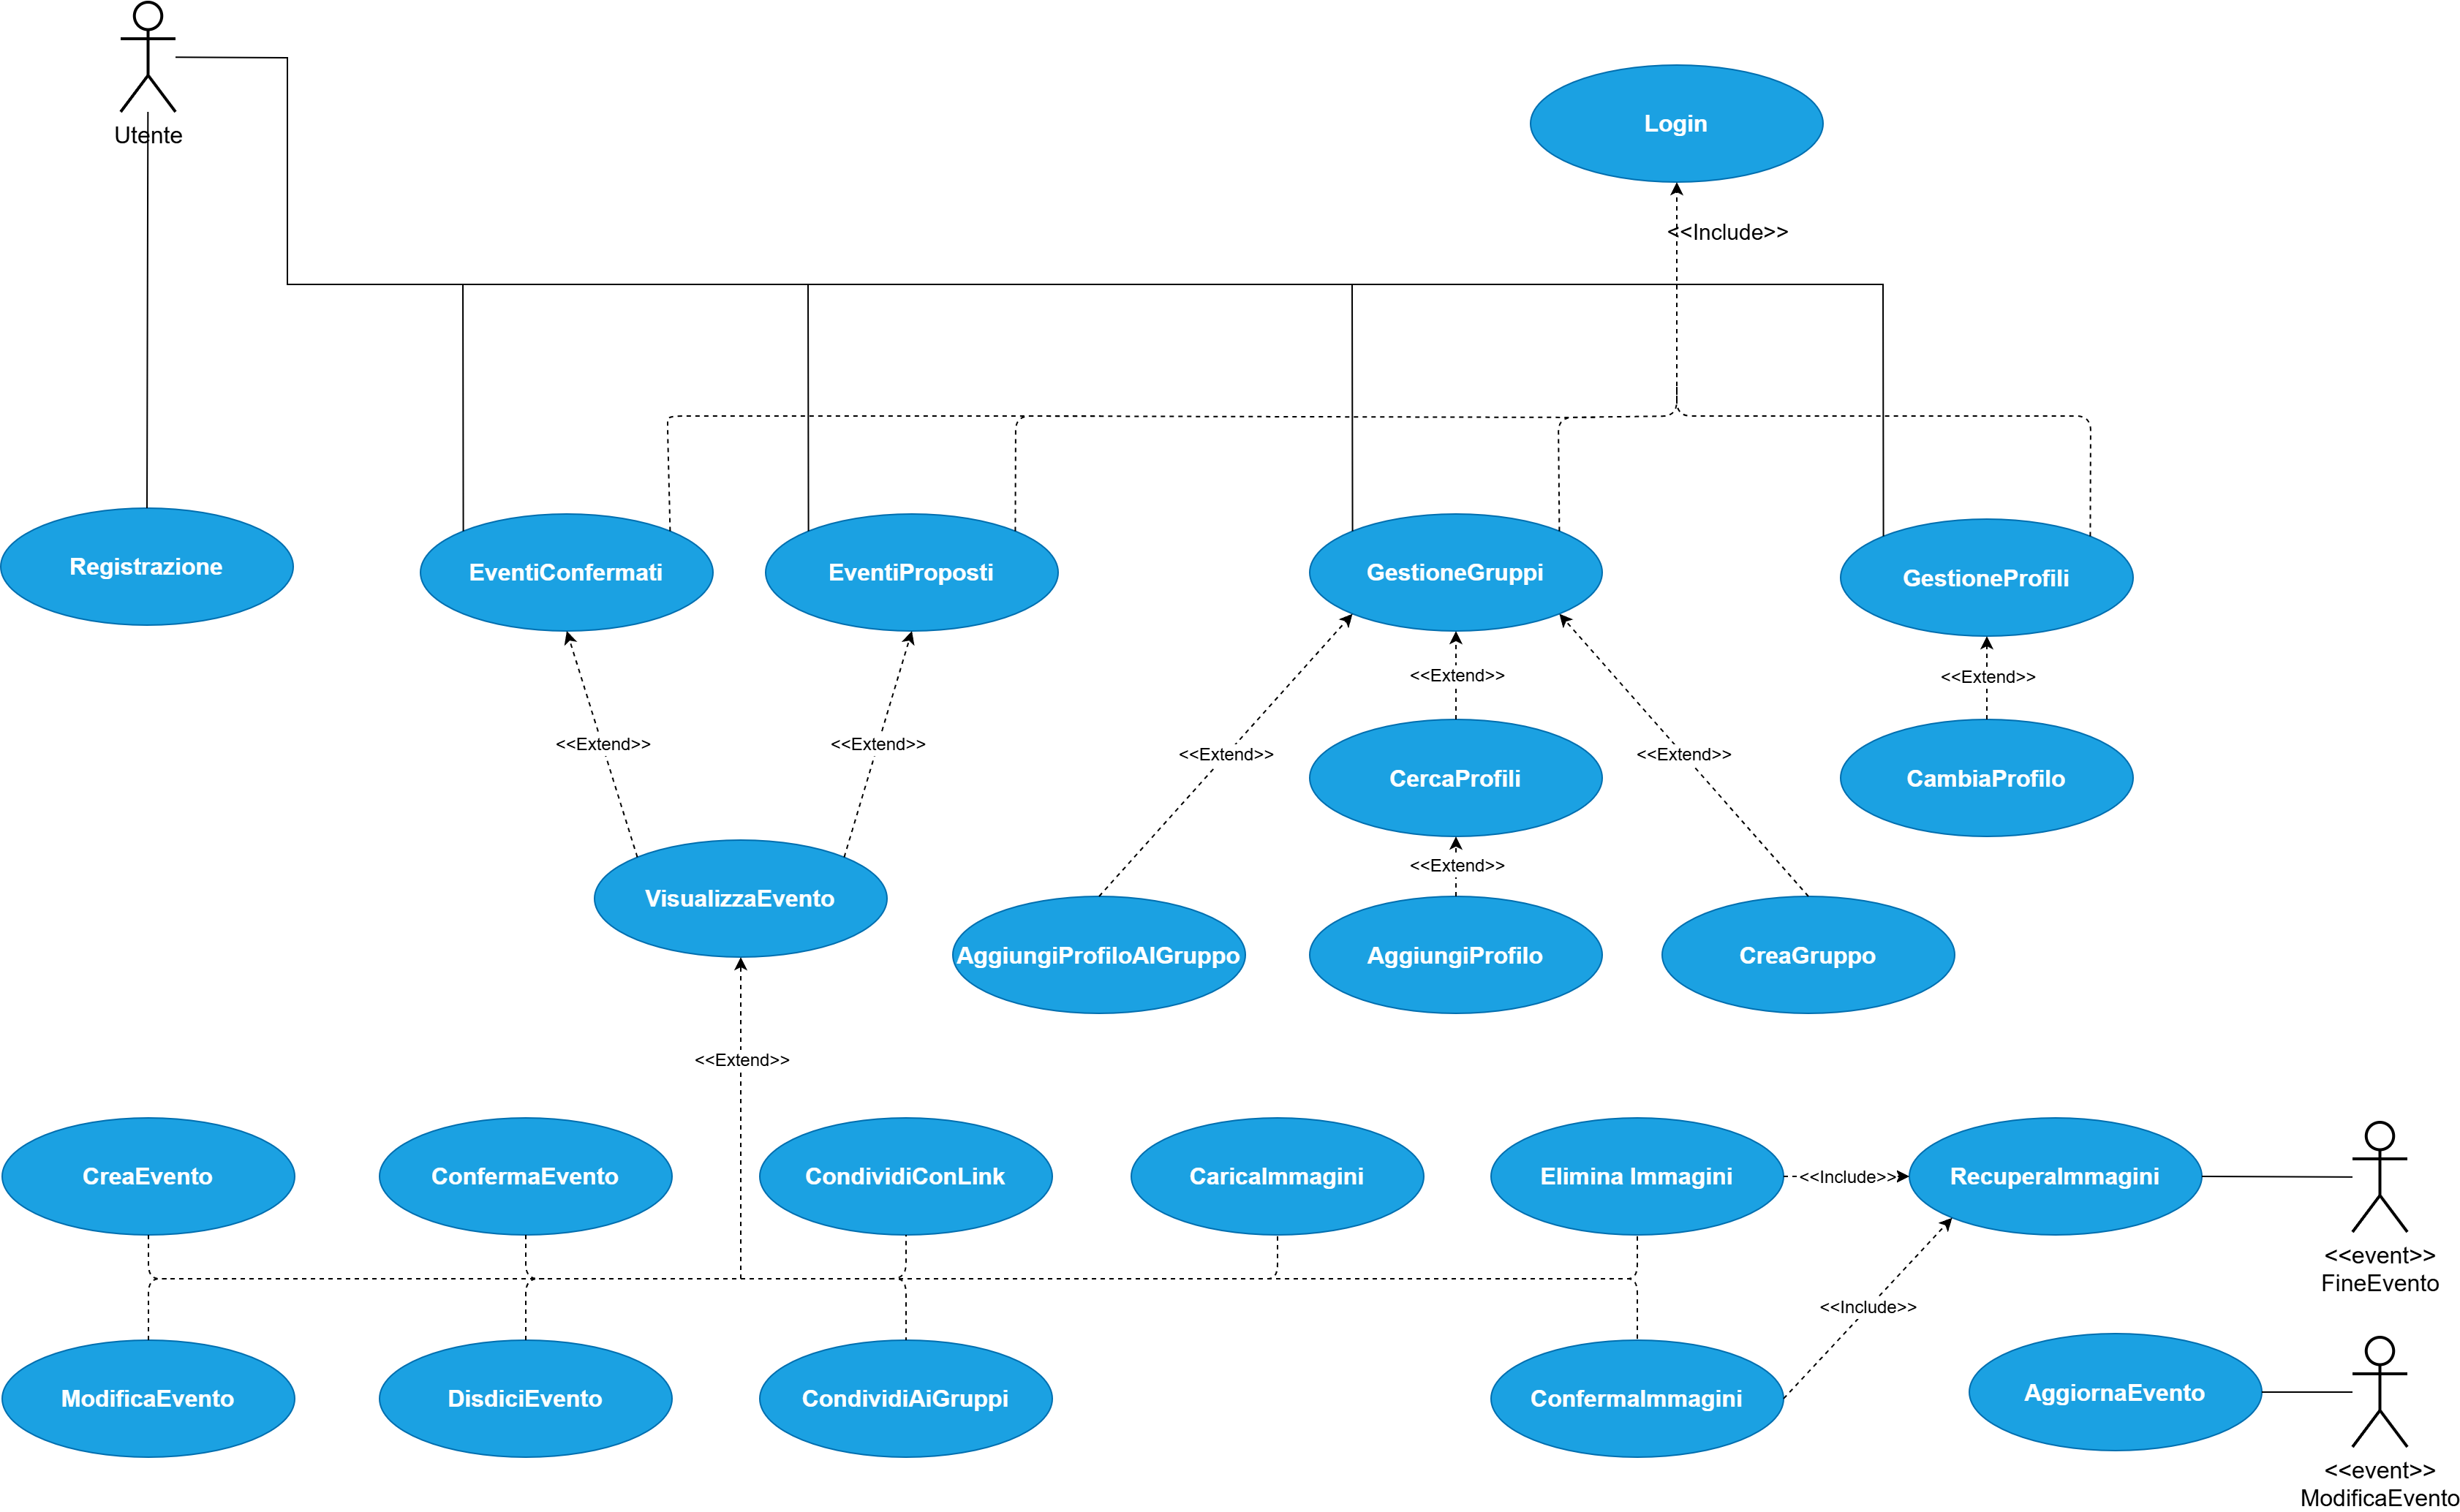
\includegraphics{Casiduso.png}}
\end{figure}

\newpage %optional
\subsubsection{Scenari}
\hfill \break

%Registrazione
\begin{tabular} {|P{4.5cm}|P{11cm}|}
  \hline
  \textbf{Titolo}                   & Registrazione                                                                            \\
  \hline
  \textbf{Descrizione}              & L'utente si registra al servizio                                                         \\
  \hline
  \textbf{Attori}                   & Utente                                                                                   \\
  \hline
  \textbf{Relazioni}                &                                                                                          \\
  \hline
  \textbf{Precondizioni}            &                                                                                          \\
  \hline
  \textbf{Postcondizioni}           & L'utente è registrato nel sistema e può interagire con il resto dell'applicazione        \\
  \hline
  \textbf{Scenario principale}      &
  1. L'utente accede alla sezione diregistrazione \linebreak
  2. L'utente inserisce email e  password \linebreak
  3. L'utente termina la registrazione, se avvenuta con successo viene reindirizzato alla pagina principale                    \\
  \hline
  \textbf{Scenari Alternativi}      &
  3. Il sistema verifica che è già presente un account con la mail inserita, quindi procede con la procedura di login normale. \\
  \hline
  \textbf{Requisiti non funzionali} &
  Per interagire l’utente deve essere autenticato \linebreak
  Velocità in lettura e scrittura dei dati                                                                                     \\
  \hline
  \textbf{Punti aperti}             &                                                                                          \\
  \hline
\end{tabular}
\hfill
\break

%Login
\begin{tabular} {|P{4.5cm}|P{11cm}|}
  \hline
  \textbf{Titolo}                   & Login                                                              \\
  \hline
  \textbf{Descrizione}              & Permette di accedere al sistema                                    \\
  \hline
  \textbf{Attori}                   & Utente                                                             \\
  \hline
  \textbf{Relazioni}                & EventiConfermati, EventiProposti, GestioneGruppi, GestioneProfili  \\
  \hline
  \textbf{Precondizioni}            &                                                                    \\
  \hline
  \textbf{Postcondizioni}           & L'utente ha accesso al sistema, limitato in base ai suoi privilegi \\
  \hline
  \textbf{Scenario principale}      & 1. L'utente inserisce le credenziali di
  accesso \linebreak 2. Il sistema verifica le credenziali \linebreak 3. Se le
  credenziali sono corrette, viene presentata la schermata iniziale                                      \\
  \hline
  \textbf{Scenari Alternativi}      & 1. L'utente inserisce le
  credenziali di accesso \linebreak 2. Il sistema verifica le credenziali
  \linebreak 3. Il sistema non riconosce le credenziali e rispedisce l'utente
  alla schermata di login con un messaggio di errore                                                     \\
  \hline
  \textbf{Requisiti non funzionali} & Velocità in lettura e scrittura dei dati\linebreak                 \\
  \hline
  \textbf{Punti aperti}             &                                                                    \\
  \hline
\end{tabular}
\hfill
\break

%EventiConfermati
\begin{tabular} {|P{4.5cm}|P{11cm}|}
  \hline
  \textbf{Titolo}                   & EventiConfermati                                            \\
  \hline
  \textbf{Descrizione}              & Viene mostrato l'elenco degli eventi confermati dall'utente \\
  \hline
  \textbf{Attori}                   & Utente                                                      \\
  \hline
  \textbf{Relazioni}                & Login, VisualizzaEvento                                     \\
  \hline
  \textbf{Precondizioni}            &                                                             \\
  \hline
  \textbf{Postcondizioni}           & Viene mostrato l'elenco degli eventi confermati             \\
  \hline
  \textbf{Scenario Principale}      & 1. L'utente va nella schermata di
  visualizzazione eventi confermati \linebreak 2. Il sistema recupera l'elenco degli eventi confermati \linebreak 3. Il sistema mostra a video
  l'elenco richiesto                                                                              \\
  \hline
  \textbf{Scenari Alternativi}      &                                                             \\
  \hline
  \textbf{Requisiti non funzionali} & Velocità di richiesta iniziale dei dati\linebreak
  Semplicità e fluidità dell'interfaccia grafica                                                  \\
  \hline
  \textbf{Punti aperti}             &                                                             \\
  \hline
\end{tabular}
\hfill
\break

%EventiProposti
\begin{tabular} {|P{4.5cm}|P{11cm}|}
  \hline
  \textbf{Titolo}                   & EventiProposti                                                           \\
  \hline
  \textbf{Descrizione}              & Viene mostrato l'elenco degli eventi proposti non confermati dall'utente \\
  \hline
  \textbf{Attori}                   & Utente                                                                   \\
  \hline
  \textbf{Relazioni}                & Login, VisualizzaEvento                                                  \\
  \hline
  \textbf{Precondizioni}            &                                                                          \\
  \hline
  \textbf{Postcondizioni}           & Viene mostrato l'elenco degli eventi proposti non confermati             \\
  \hline
  \textbf{Scenario Principale}      & 1. L'utente va nella schermata di
  visualizzazione eventi proposti \linebreak 2. Il sistema recupera l'elenco degli eventi proposti non confermati \linebreak 3. Il sistema mostra a video
  l'elenco richiesto                                                                                           \\
  \hline
  \textbf{Scenari Alternativi}      &                                                                          \\
  \hline
  \textbf{Requisiti non funzionali} & Velocità di richiesta iniziale dei dati\linebreak
  Semplicità e fluidità dell'interfaccia grafica                                                               \\
  \hline
  \textbf{Punti aperti}             &                                                                          \\
  \hline
\end{tabular}
\hfill
\break

%VisualizzaEvento
\begin{tabular} {|P{4.5cm}|P{11cm}|}
  \hline
  \textbf{Titolo}                   & VisualizzaEvento                                                                                                                                                                                   \\
  \hline
  \textbf{Descrizione}              & Viene mostrato l'evento con i suoi dettagli, con la possibilità di modificarli                                                                                                                     \\
  \hline
  \textbf{Attori}                   & Utente                                                                                                                                                                                             \\
  \hline
  \textbf{Relazioni}                & EventiConfermati, EventiProposti, CreaEvento, ModificaEvento, ConfermaEvento, DisdiciEvento, CondividiConLink, CondividiAiGruppi, CaricaImmagini, EliminaImmagini, ConfermaImmagini                \\
  \hline
  \textbf{Precondizioni}            &                                                                                                                                                                                                    \\
  \hline
  \textbf{Postcondizioni}           & Viene mostrato l'evento e i suoi dettagli, le modifiche vengono temporaneamente salvate                                                                                                            \\
  \hline
  \textbf{Scenario Principale}      & 1. L'utente seleziona un evento \linebreak 2. Il sistema recupera i dati dell'evento \linebreak 3. Il sistema mostra a video i dati dell'evento da la possibilità di modificare i dati dell'evento \\
  \hline
  \textbf{Scenari Alternativi}      & Scenario alternativo A: \linebreak
  1. L'utente seleziona l'opzione di creare un nuovo evento \linebreak 2. Il sistema mostra a video i dati dell'evento da la possibilità di modificare i dati dell'evento         \linebreak
  Scenario alternativo B:\linebreak
  1. L'utente viene indirizzato tramite link\linebreak
  2. Il sistema recupera i dati dell'evento\linebreak
  3. Il sistema mostra a video i dati dell'evento da la possibilità di modificare i dati dell'evento                                                                                                                                     \\
  \hline
  \textbf{Requisiti non funzionali} & Velocità in lettura e scrittura dei dati\linebreak
  Semplicità e fluidità dell'interfaccia grafica                                                                                                                                                                                         \\
  \hline
  \textbf{Punti aperti}             &                                                                                                                                                                                                    \\
  \hline
\end{tabular}
\hfill
\break

%CreaEvento
\begin{tabular} {|P{4.5cm}|P{11cm}|}
  \hline
  \textbf{Titolo}                   & CreaEvento                                                                        \\
  \hline
  \textbf{Descrizione}              & Crea un evento e lo aggiunge                                                      \\
  \hline
  \textbf{Attori}                   & Utente                                                                            \\
  \hline
  \textbf{Relazioni}                & VisualizzaEvento                                                                  \\
  \hline
  \textbf{Precondizioni}            & L'evento non esiste, i dati inseriti sono corretti                                \\
  \hline
  \textbf{Postcondizioni}           & Viene creato l'evento e visualizzato nella pagina relativa                        \\
  \hline
  \textbf{Scenario Principale}      & 1. VisualizzaEvento \linebreak
  2. Il sistema controlla che i dati inseriti siano corretti\linebreak
  3. Se i dati sono corretti, l'evento viene salvato\linebreak
  4. L'evento è visualizzato nella schermata degli eventi\linebreak
  5. Tutti i dispositivi collegati al profilo visualizzano l'evento                                                     \\
  \hline
  \textbf{Scenari Alternativi}      & 3. Se i dati risultano sbagliati, il sistema notifica l'utente indicando l'errore \\
  \hline
  \textbf{Requisiti non funzionali} & Velocità in lettura e scrittura dei dati                                          \\
  \hline
  \textbf{Punti aperti}             &                                                                                   \\
  \hline
\end{tabular}
\hfill
\break

%ModificaEvento
\begin{tabular} {|P{4.5cm}|P{11cm}|}
  \hline
  \textbf{Titolo}                   & ModificaEvento                                                                    \\
  \hline
  \textbf{Descrizione}              & Salva le modifiche ad un evento                                                   \\
  \hline
  \textbf{Attori}                   & Utente                                                                            \\
  \hline
  \textbf{Relazioni}                & VisualizzaEvento                                                                  \\
  \hline
  \textbf{Precondizioni}            & L'evento esiste e sono stati modificati dei dati                                  \\
  \hline
  \textbf{Postcondizioni}           & Le modifiche vengono salvate e propagate a tutti i profili collegati              \\
  \hline
  \textbf{Scenario Principale}      & 1. VisualizzaEvento \linebreak
  2. Il sistema controlla che i dati modificati siano corretti\linebreak
  3. Le immagini vengono salvate\linebreak
  4. Tutti i dispositivi collegati ai profili collegati all'evento visualizzano le immagini                             \\
  \hline
  \textbf{Scenari Alternativi}      & 3. Se i dati risultano sbagliati, il sistema notifica l'utente indicando l'errore \\
  \hline
  \textbf{Requisiti non funzionali} & Velocità in lettura e scrittura dei dati                                          \\
  \hline
  \textbf{Punti aperti}             &                                                                                   \\
  \hline
\end{tabular}
\hfill
\break

%ConfermaEvento
\begin{tabular} {|P{4.5cm}|P{11cm}|}
  \hline
  \textbf{Titolo}                   & ConfermaEvento                                                                                                                       \\
  \hline
  \textbf{Descrizione}              & Conferma la partecipazione ad un evento                                                                                              \\
  \hline
  \textbf{Attori}                   & Utente                                                                                                                               \\
  \hline
  \textbf{Relazioni}                & VisualizzaEvento                                                                                                                     \\
  \hline
  \textbf{Precondizioni}            & L'evento esiste e il profilo corrente non lo ha confermato                                                                           \\
  \hline
  \textbf{Postcondizioni}           & Il profilo conferma la sua presenza, tutti i profili collegati vengono aggiornati, l'evento è visualizzato tra gli eventi confermati \\
  \hline
  \textbf{Scenario Principale}      & 1. VisualizzaEvento \linebreak
  2. L'utente conferma la sua presenza\linebreak
  3. L'evento è visualizzato tra gli eventi confermati\linebreak
  4. Tutti i dispositivi collegati ai profili collegati all'evento visualizzano l'aggiornamento                                                                            \\
  \hline
  \textbf{Scenari Alternativi}      &                                                                                                                                      \\
  \hline
  \textbf{Requisiti non funzionali} & Velocità in lettura e scrittura dei dati                                                                                             \\
  \hline
  \textbf{Punti aperti}             &                                                                                                                                      \\
  \hline
\end{tabular}
\hfill
\break

%DisdiciEvento
\begin{tabular} {|P{4.5cm}|P{11cm}|}
  \hline
  \textbf{Titolo}                   & DisdiciEvento                                                                                                                     \\
  \hline
  \textbf{Descrizione}              & Disdice la partecipazione ad un evento                                                                                            \\
  \hline
  \textbf{Attori}                   & Utente                                                                                                                            \\
  \hline
  \textbf{Relazioni}                & VisualizzaEvento                                                                                                                  \\
  \hline
  \textbf{Precondizioni}            & L'evento esiste e il profilo corrente lo ha confermato                                                                            \\
  \hline
  \textbf{Postcondizioni}           & Il profilo disdice la sua presenza, tutti i profili collegati vengono aggiornati, l'evento è visualizzato tra gli eventi proposti \\
  \hline
  \textbf{Scenario Principale}      & 1. VisualizzaEvento \linebreak
  2. L'utente disdice la sua presenza\linebreak
  3. L'evento è visualizzato tra gli eventi proposti\linebreak
  4. Tutti i dispositivi collegati ai profili collegati all'evento visualizzano l'aggiornamento                                                                         \\
  \hline
  \textbf{Scenari Alternativi}      &                                                                                                                                   \\
  \hline
  \textbf{Requisiti non funzionali} & Velocità in lettura e scrittura dei dati                                                                                          \\
  \hline
  \textbf{Punti aperti}             &                                                                                                                                   \\
  \hline
\end{tabular}
\hfill
\break

%CaricaImmagini
\begin{tabular} {|P{4.5cm}|P{11cm}|}
  \hline
  \textbf{Titolo}                   & CaricaImmagini                                                                  \\
  \hline
  \textbf{Descrizione}              & Permette all'utente di selezionare immagini da collegare all'evento, salvandole \\
  \hline
  \textbf{Attori}                   & Utente                                                                          \\
  \hline
  \textbf{Relazioni}                & VisualizzaEvento                                                                \\
  \hline
  \textbf{Precondizioni}            & L'evento esiste                                                                 \\
  \hline
  \textbf{Postcondizioni}           & Le immagini vengono salvate e propagate a tutti i profili collegati             \\
  \hline
  \textbf{Scenario Principale}      & 1. VisualizzaEvento \linebreak
  2. L'utente seleziona le immagini che vuole caricare\linebreak
  3. Le immagini vengono salvate\linebreak
  4. Tutti i dispositivi collegati ai profili collegati all'evento visualizzano le immagini                           \\
  \hline
  \textbf{Scenari Alternativi}      &                                                                                 \\
  \hline
  \textbf{Requisiti non funzionali} & Velocità in lettura e scrittura dei dati\linebreak
  Semplicità e fluidità dell'interfaccia grafica                                                                      \\
  \hline
  \textbf{Punti aperti}             &                                                                                 \\
  \hline
\end{tabular}
\hfill
\break

%RecuperaImmagini
\begin{tabular} {|P{4.5cm}|P{11cm}|}
  \hline
  \textbf{Titolo}                   & RecuperaImmagini                                                          \\
  \hline
  \textbf{Descrizione}              & Controlla la galleria e salva in locale le foto scattate durante l'evento \\
  \hline
  \textbf{Attori}                   & FineEvento                                                                \\
  \hline
  \textbf{Relazioni}                & EliminaImmagini, ConfermaImmagini                                         \\
  \hline
  \textbf{Precondizioni}            & L'evento esiste ed è concluso                                             \\
  \hline
  \textbf{Postcondizioni}           & Le immagini vengono salvate in locale e l'utente viene notificato         \\
  \hline
  \textbf{Scenario Principale}      & 1. Il sistema controlla che l'evento sia finito \linebreak
  2. Il sistema controlla la galleria per trovare le immagini scattate nell'arco temporale dell'evento\linebreak
  3. Se ci sono immagini, vengono salvate in locale e l'utente viene notificato                                 \\
  \hline
  \textbf{Scenari Alternativi}      &                                                                           \\
  \hline
  \textbf{Requisiti non funzionali} & Velocità in lettura e scrittura dei dati                                  \\
  \hline
  \textbf{Punti aperti}             &                                                                           \\
  \hline
\end{tabular}
\hfill
\break

%EliminaImmagini
\begin{tabular} {|P{4.5cm}|P{11cm}|}
  \hline
  \textbf{Titolo}                   & EliminaImmagini                                       \\
  \hline
  \textbf{Descrizione}              & Rimuove le immagini dall'evento                       \\
  \hline
  \textbf{Attori}                   & Utente                                                \\
  \hline
  \textbf{Relazioni}                & RecuperaImmagini, VisualizzaEvento                    \\
  \hline
  \textbf{Precondizioni}            & L'evento esiste ed esistono immagini collegate        \\
  \hline
  \textbf{Postcondizioni}           & Le immagini selezionate vengono rimosse dall'evento   \\
  \hline
  \textbf{Scenario Principale}      & 1.VisualizzaEvento
  1. L'utente seleziona le immagini caricate automaticamente da eliminare\linebreak
  1. Le immagini vengono rimosse dall'evento                                                \\
  \hline
  \textbf{Scenari Alternativi}      & 1. VisualizzaEvento \linebreak
  2. L'utente seleziona le immagini da eliminare\linebreak
  3. Le immagini vengono rimosse dall'evento, e le modifiche propagate ai profili collegati \\
  \hline
  \textbf{Requisiti non funzionali} &                                                       \\
  \hline
  \textbf{Punti aperti}             &                                                       \\
  \hline
\end{tabular}
\hfill
\break

%ConfermaImmagini
\begin{tabular} {|P{4.5cm}|P{11cm}|}
  \hline
  \textbf{Titolo}                   & ConfermaImmagini                                              \\
  \hline
  \textbf{Descrizione}              & L'utente conferma le immagini caricate automaticamente        \\
  \hline
  \textbf{Attori}                   & Utente                                                        \\
  \hline
  \textbf{Relazioni}                & RecuperaImmagini, VisualizzaEvento                            \\
  \hline
  \textbf{Precondizioni}            & L'evento esiste ed esistono immagini caricate automaticamente \\
  \hline
  \textbf{Postcondizioni}           & Le immagini selezionate vengono condivise con l'evento        \\
  \hline
  \textbf{Scenario Principale}      & 1. VisualizzaEvento \linebreak
  2. L'utente seleziona conferma le immagini caricate automaticamente\linebreak
  3. Le immagini vengono aggiunte all'evento e tutti i profili collegati visualizzano le modifiche  \\
  \hline
  \textbf{Scenari Alternativi}      &                                                               \\
  \hline
  \textbf{Requisiti non funzionali} & Velocità in lettura e scrittura dei dati                      \\
  \hline
  \textbf{Punti aperti}             &                                                               \\
  \hline
\end{tabular}
\hfill
\break

%CondividiAiGruppi
\begin{tabular} {|P{4.5cm}|P{11cm}|}
  \hline
  \textbf{Titolo}                   & CondividiAiGruppi                                                           \\
  \hline
  \textbf{Descrizione}              & Permette di condividere l'evento ai gruppi                                  \\
  \hline
  \textbf{Attori}                   & Utente                                                                      \\
  \hline
  \textbf{Relazioni}                & VisualizzaEvento                                                            \\
  \hline
  \textbf{Precondizioni}            & L'evento esiste                                                             \\
  \hline
  \textbf{Postcondizioni}           & L'evento è condiviso con tutti i profili appartenenti ai gruppi selezionati \\
  \hline
  \textbf{Scenario Principale}      & 1. VisualizzaEvento\linebreak
  2. Il sistema visualizza l'elenco dei gruppi di cui l'utente fa parte, permettendone la selezione\linebreak
  3. L'evento è condiviso con tutti i profili dei gruppi selezionati, che visualizzeranno l'evento tra i proposti \\
  \hline
  \textbf{Scenari Alternativi}      &                                                                             \\
  \hline
  \textbf{Requisiti non funzionali} & Velocità in lettura e scrittura dei dati                                    \\
  \hline
  \textbf{Punti aperti}             &                                                                             \\
  \hline
\end{tabular}
\hfill
\break

%CondividiConLink
\begin{tabular} {|P{4.5cm}|P{11cm}|}
  \hline
  \textbf{Titolo}                   & CondividiConLink                                  \\
  \hline
  \textbf{Descrizione}              & Permette di condividere l'evento tramite link     \\
  \hline
  \textbf{Attori}                   & Utente                                            \\
  \hline
  \textbf{Relazioni}                & VisualizzaEvento                                  \\
  \hline
  \textbf{Precondizioni}            & L'evento esiste                                   \\
  \hline
  \textbf{Postcondizioni}           & L'utente ottiene un link che può confidividere    \\
  \hline
  \textbf{Scenario Principale}      & 1. VisualizzaEvento\linebreak
  2. Il sistema mostra le opzioni di condivisione del link                              \\
  \hline
  \textbf{Scenari Alternativi}      & 2. Il sistema salva il link in memoria temporanea \\
  \hline
  \textbf{Requisiti non funzionali} & Velocità in lettura e scrittura dei dati          \\
  \hline
  \textbf{Punti aperti}             &                                                   \\
  \hline
\end{tabular}
\hfill
\break

%AggiornaEvento
\begin{tabular} {|P{4.5cm}|P{11cm}|}
  \hline
  \textbf{Titolo}                   & AggiornaEvento                                                                  \\
  \hline
  \textbf{Descrizione}              & Aggiorna l’evento in locale in base alle modifiche apportate da profili esterni \\
  \hline
  \textbf{Attori}                   & ModificaEvento                                                                  \\
  \hline
  \textbf{Relazioni}                &                                                                                 \\
  \hline
  \textbf{Precondizioni}            & L'evento esiste ed è cdondiviso con uno dei profili collegati all'utente        \\
  \hline
  \textbf{Postcondizioni}           & L'evento viene aggiornato con le modifiche                                      \\
  \hline
  \textbf{Scenario Principale}      & 1. Il sistema riceve la notifica che un evento è stato modificato \linebreak
  2. Il sistema recupera le modifiche e aggiorna l'evento di conseguenza                                              \\
  \hline
  \textbf{Scenari Alternativi}      &                                                                                 \\
  \hline
  \textbf{Requisiti non funzionali} & Velocità in lettura e scrittura dei dati\                                       \\
  \hline
  \textbf{Punti aperti}             &                                                                                 \\
  \hline
\end{tabular}
\hfill
\break

%GestioneGruppi
\begin{tabular} {|P{4.5cm}|P{11cm}|}
  \hline
  \textbf{Titolo}                   & GestioneGruppi                                                        \\
  \hline
  \textbf{Descrizione}              & Viene mostrato l'elenco dei gruppi appartenenti al profilo corrente   \\
  \hline
  \textbf{Attori}                   & Utente                                                                \\
  \hline
  \textbf{Relazioni}                & Login, CercaProfili, CreaGruppo                                       \\
  \hline
  \textbf{Precondizioni}            &                                                                       \\
  \hline
  \textbf{Postcondizioni}           & Viene mostrato l'elenco degli gruppi appartenenti al profilo corrente \\
  \hline
  \textbf{Scenario Principale}      & 1. L'utente va nella schermata di gestione gruppi \linebreak
  2. Il sistema recupera l'elenco dei gruppi appartenenti al profilo corrente \linebreak
  3. Il sistema mostra a video l'elenco richiesto                                                           \\
  \hline
  \textbf{Scenari Alternativi}      &                                                                       \\
  \hline
  \textbf{Requisiti non funzionali} & Velocità di richiesta iniziale dei dati\linebreak
  Semplicità e fluidità dell'interfaccia grafica                                                            \\
  \hline
  \textbf{Punti aperti}             &                                                                       \\
  \hline
\end{tabular}
\hfill
\break

%CercaProfili
\begin{tabular} {|P{4.5cm}|P{11cm}|}
  \hline
  \textbf{Titolo}                   & CercaProfili                                              \\
  \hline
  \textbf{Descrizione}              & L'utente cerca i profili tramite tag                      \\
  \hline
  \textbf{Attori}                   & Utente                                                    \\
  \hline
  \textbf{Relazioni}                & GestioneGruppi, AggiungiProfilo                           \\
  \hline
  \textbf{Precondizioni}            &                                                           \\
  \hline
  \textbf{Postcondizioni}           & Si visualizza la lista dei profili con tag corrispondente \\
  \hline
  \textbf{Scenario principale}      & 1. GestioneGruppi \linebreak
  2. L'utente inserisce il tag parziale o completo del profilo per cui eseguire la ricerca \linebreak
  3. Il sistema ottiene la lista dei profili che corrispondono alla ricerca\linebreak
  4. La lista viene mostrata all'utente                                                         \\
  \hline
  \textbf{Scenari Alternativi}      &                                                           \\
  \hline
  \textbf{Requisiti non funzionali} & Velocità in lettura e scrittura dei dati\linebreak
  Semplicità e fluidità dell'interfaccia grafica                                                \\
  \hline
  \textbf{Punti aperti}             &                                                           \\
  \hline
\end{tabular}
\hfill
\break

%AggiungiProfilo
\begin{tabular} {|P{4.5cm}|P{11cm}|}
  \hline
  \textbf{Titolo}                   & AggiungiProfilo                                                  \\
  \hline
  \textbf{Descrizione}              & si aggiunge il profilo selezionato alla lista gruppi del profilo \\
  \hline
  \textbf{Attori}                   & Utente                                                           \\
  \hline
  \textbf{Relazioni}                & CercaProfili                                                     \\
  \hline
  \textbf{Precondizioni}            & Il profilo selezionato esiste                                    \\
  \hline
  \textbf{Postcondizioni}           & Il profilo selezionato è visibile tra la lista dei gruppi        \\
  \hline
  \textbf{Scenario principale}      & 1. CercaProfili \linebreak
  2. L'utente seleziona il profilo da aggiungere \linebreak
  3. Il profilo viene aggiunto nella lista dei gruppi\linebreak                                        \\
  \hline
  \textbf{Scenari Alternativi}      &                                                                  \\
  \hline
  \textbf{Requisiti non funzionali} & Velocità in lettura e scrittura dei dati                         \\
  \hline
  \textbf{Punti aperti}             &                                                                  \\
  \hline
\end{tabular}
\hfill
\break

%CreaGruppo
\begin{tabular} {|P{4.5cm}|P{11cm}|}
  \hline
  \textbf{Titolo}                   & CreaGruppo                                                                          \\
  \hline
  \textbf{Descrizione}              & L'utente crea un gruppo                                                             \\
  \hline
  \textbf{Attori}                   & Utente                                                                              \\
  \hline
  \textbf{Relazioni}                & GestioneGruppi, AggiungiProfiloAlGruppo                                             \\
  \hline
  \textbf{Precondizioni}            &                                                                                     \\
  \hline
  \textbf{Postcondizioni}           & Il gruppo è creato ed aggiunto alla lista dei gruppi di tutti i profili interessati \\
  \hline
  \textbf{Scenario principale}      & 1. GestioneGruppi \linebreak
  2. L'utente inserisce il nome ed eventualmente i profili interessati \linebreak
  3. Il sistema crea il gruppo e lo aggiunge alla lista dei gruppi di tutti i profili interessati\linebreak               \\
  \hline
  \textbf{Scenari Alternativi}      &                                                                                     \\
  \hline
  \textbf{Requisiti non funzionali} & Velocità in lettura e scrittura dei dati                                            \\
  \hline
  \textbf{Punti aperti}             &                                                                                     \\
  \hline
\end{tabular}
\hfill
\break

%AggiungiProfiloAlGruppo
\begin{tabular} {|P{4.5cm}|P{11cm}|}
  \hline
  \textbf{Titolo}                   & AggiungiProfiloAlGruppo                                          \\
  \hline
  \textbf{Descrizione}              & si aggiunge il profilo selezionato alla lista gruppi del profilo \\
  \hline
  \textbf{Attori}                   & Utente                                                           \\
  \hline
  \textbf{Relazioni}                & GestioneGruppi                                                   \\
  \hline
  \textbf{Precondizioni}            & Il profilo selezionato esiste                                    \\
  \hline
  \textbf{Postcondizioni}           & Il profilo selezionato è tra la lista i profili del gruppo       \\
  \hline
  \textbf{Scenario principale}      & 1. GestioneGruppi \linebreak
  2. L'utente seleziona il profilo da aggiungere\linebreak
  3. Il sistema aggiunge il profilo alla lista dei profili del gruppo\linebreak
  4. Il profilo aggiunto visualizza il gruppo nella sua lista dei gruppi                               \\
  \hline
  \textbf{Scenari Alternativi}      &                                                                  \\
  \hline
  \textbf{Requisiti non funzionali} & Velocità in lettura e scrittura dei dati                         \\
  \hline
  \textbf{Punti aperti}             &                                                                  \\
  \hline
\end{tabular}
\hfill
\break

%GestioneProfili
\begin{tabular} {|P{4.5cm}|P{11cm}|}
  \hline
  \textbf{Titolo}                   & GestioneProfili                                               \\
  \hline
  \textbf{Descrizione}              & Viene mostrato l'elenco dei profili collegati all'utente      \\
  \hline
  \textbf{Attori}                   & Utente                                                        \\
  \hline
  \textbf{Relazioni}                & Login, CambiaProfilo                                          \\
  \hline
  \textbf{Precondizioni}            &                                                               \\
  \hline
  \textbf{Postcondizioni}           & Viene mostrato l'elenco degli profili collegati all'utente    \\
  \hline
  \textbf{Scenario Principale}      & 1. L'utente va nella schermata di gestione profili \linebreak
  2. Il sistema recupera l'elenco dei profili collegati all'utente \linebreak
  3. Il sistema mostra a video l'elenco richiesto                                                   \\
  \hline
  \textbf{Scenari Alternativi}      &                                                               \\
  \hline
  \textbf{Requisiti non funzionali} & Velocità di richiesta iniziale dei dati\linebreak
  Semplicità e fluidità dell'interfaccia grafica                                                    \\
  \hline
  \textbf{Punti aperti}             &                                                               \\
  \hline
\end{tabular}
\hfill
\break

%CambiaProfilo
\begin{tabular} {|P{4.5cm}|P{11cm}|}
  \hline
  \textbf{Titolo}                   & CambiaProfilo                                            \\
  \hline
  \textbf{Descrizione}              & Modifica il profilo corrente con quello selezionato      \\
  \hline
  \textbf{Attori}                   & Utente                                                   \\
  \hline
  \textbf{Relazioni}                & GestioneProfili                                          \\
  \hline
  \textbf{Precondizioni}            & Il profilo selezionabile non è quello attualmente in uso \\
  \hline
  \textbf{Postcondizioni}           & Il profilo corrente è quello che è stato selezionato     \\
  \hline
  \textbf{Scenario Principale}      & 1. GestioneProfili \linebreak
  2. L'utente seleziona il profilo\linebreak
  3. Il profilo corrente diventa quello selezionato                                            \\
  \hline
  \textbf{Scenari Alternativi}      &                                                          \\
  \hline
  \textbf{Requisiti non funzionali} &                                                          \\
  \hline
  \textbf{Punti aperti}             &                                                          \\
  \hline
\end{tabular}

\clearpage

\subsection{Analisi del Rischio}

\subsubsection{Tabella Valutazione dei Beni}

\begin{tabular} {|P{3.5cm}|P{5.5cm}|P{6.7cm}|}
  \hline
  \textbf{Bene}                     & \textbf{Valore}                                                                                              & \textbf{Esposizione}      \\
  \hline
  Sistema Informativo               & Alto. Fondamentale per il funzionamento del servizio                                                         &
  Alta. Perdita finanziaria e di immagine                                                                                                                                      \\
  \hline
  Informazioni dei clienti          & Alto. Informazioni personali                                                                                 &
  Alta. Perdita di immagine dovuta alla divulgazione
  di dati sensibili                                                                                                                                                            \\
  \hline
  Informazioni relativi agli eventi & Medio-alto, necessari per offrire il servizio e contenenti informazioni personali e potenzialmente riservate &
  Molto Alta. Perdita di immagine possibile con la divulgazione dei dati relativi ai
  clienti                                                                                                                                                                      \\
  \hline
  Dati dei gruppi                   & Medio. Necessario per condividere gli eventi                                                                 & Alta. Perdita di immagine \\
  \hline
\end{tabular}

\subsubsection{Tabella Minacce/Controlli}

\begin{tabular} {|P{3cm}|P{2cm}|P{6.1cm}|P{4cm}|}
  \hline
  \textbf{Minaccia}                                 & \textbf{Probab.} & \textbf{Controllo}                                                                                                                                                                                                                      & \textbf{Fattibilità}                                              \\
  \hline
  Furto credenziali utente                          & Alta             & Controllo sulla sicurezza della password - Log delle operazioni, autenticazione a due fattori                                                                                                                                           & Costo implementativo medio                                        \\
  \hline
  Alterazione o intercettazione delle comunicazioni & Alta             & Utilizzo di un canale sicuro - Log delle operazioni, autenticazione integrata nel messaggio                                                                                                                                             & Basso costo di realizzazione con determinati protocolli           \\
  \hline
  Accesso non autorizzato al database               & Bassa            & Accesso da macchine sicure - Log di tutte le operazioni                                                                                                                                                                                 & Basso costo di realizzazione, il server deve essere ben custodito \\
  \hline
  DoS                                               & Bassa            & Controllo e limitazione delle richieste                                                                                                                                                                                                 & Media complessità di implementazione                              \\
  \hline
  Saturazione del database                          & Bassa            & 1. Limitazione delle richieste in un dato intervallo di tempo. \linebreak 2. Limitazione della grandezza delle richieste singole \linebreak 3. Limitazione della grandezza richiesta dallo stesso utente in un dato intervallo di tempo & Media complessità di implementazione                              \\
  \hline
\end{tabular}

\subsubsection{Analisi Tecnologica della Sicurezza}

\begin{tabular} {|P{4cm}|P{12cm}|}
  \hline
  Tecnologia                     & Vulnerabilità                                            \\
  \hline
  Autenticazione email/password  & • Utente rivela volontariamente la password \linebreak
  • Utente rivela la password con un attacco di ingegneria sociale \linebreak
  • Password banali                                                                         \\
  \hline
  Cifratura comunicazioni        & • In caso di cifratura simmetrica particolare
  attenzione va alla lunghezza delle chiavi ed alla loro memorizzazione                     \\
  \hline
  Architettura Client/Server     & • DoS \linebreak
  • Man in the Middle \linebreak
  • Sniffing delle comunicazioni                                                            \\
  \hline
  Connessione Server/Persistenza & • Limite massimo di connessioni contemporanee \linebreak
  • Saturazione del Database                                                                \\
  \hline
\end{tabular}

\newpage
\subsubsection{Security Use Case \& Misuse Case}
\par

\begin{figure}[h!]
  \begin{center}
    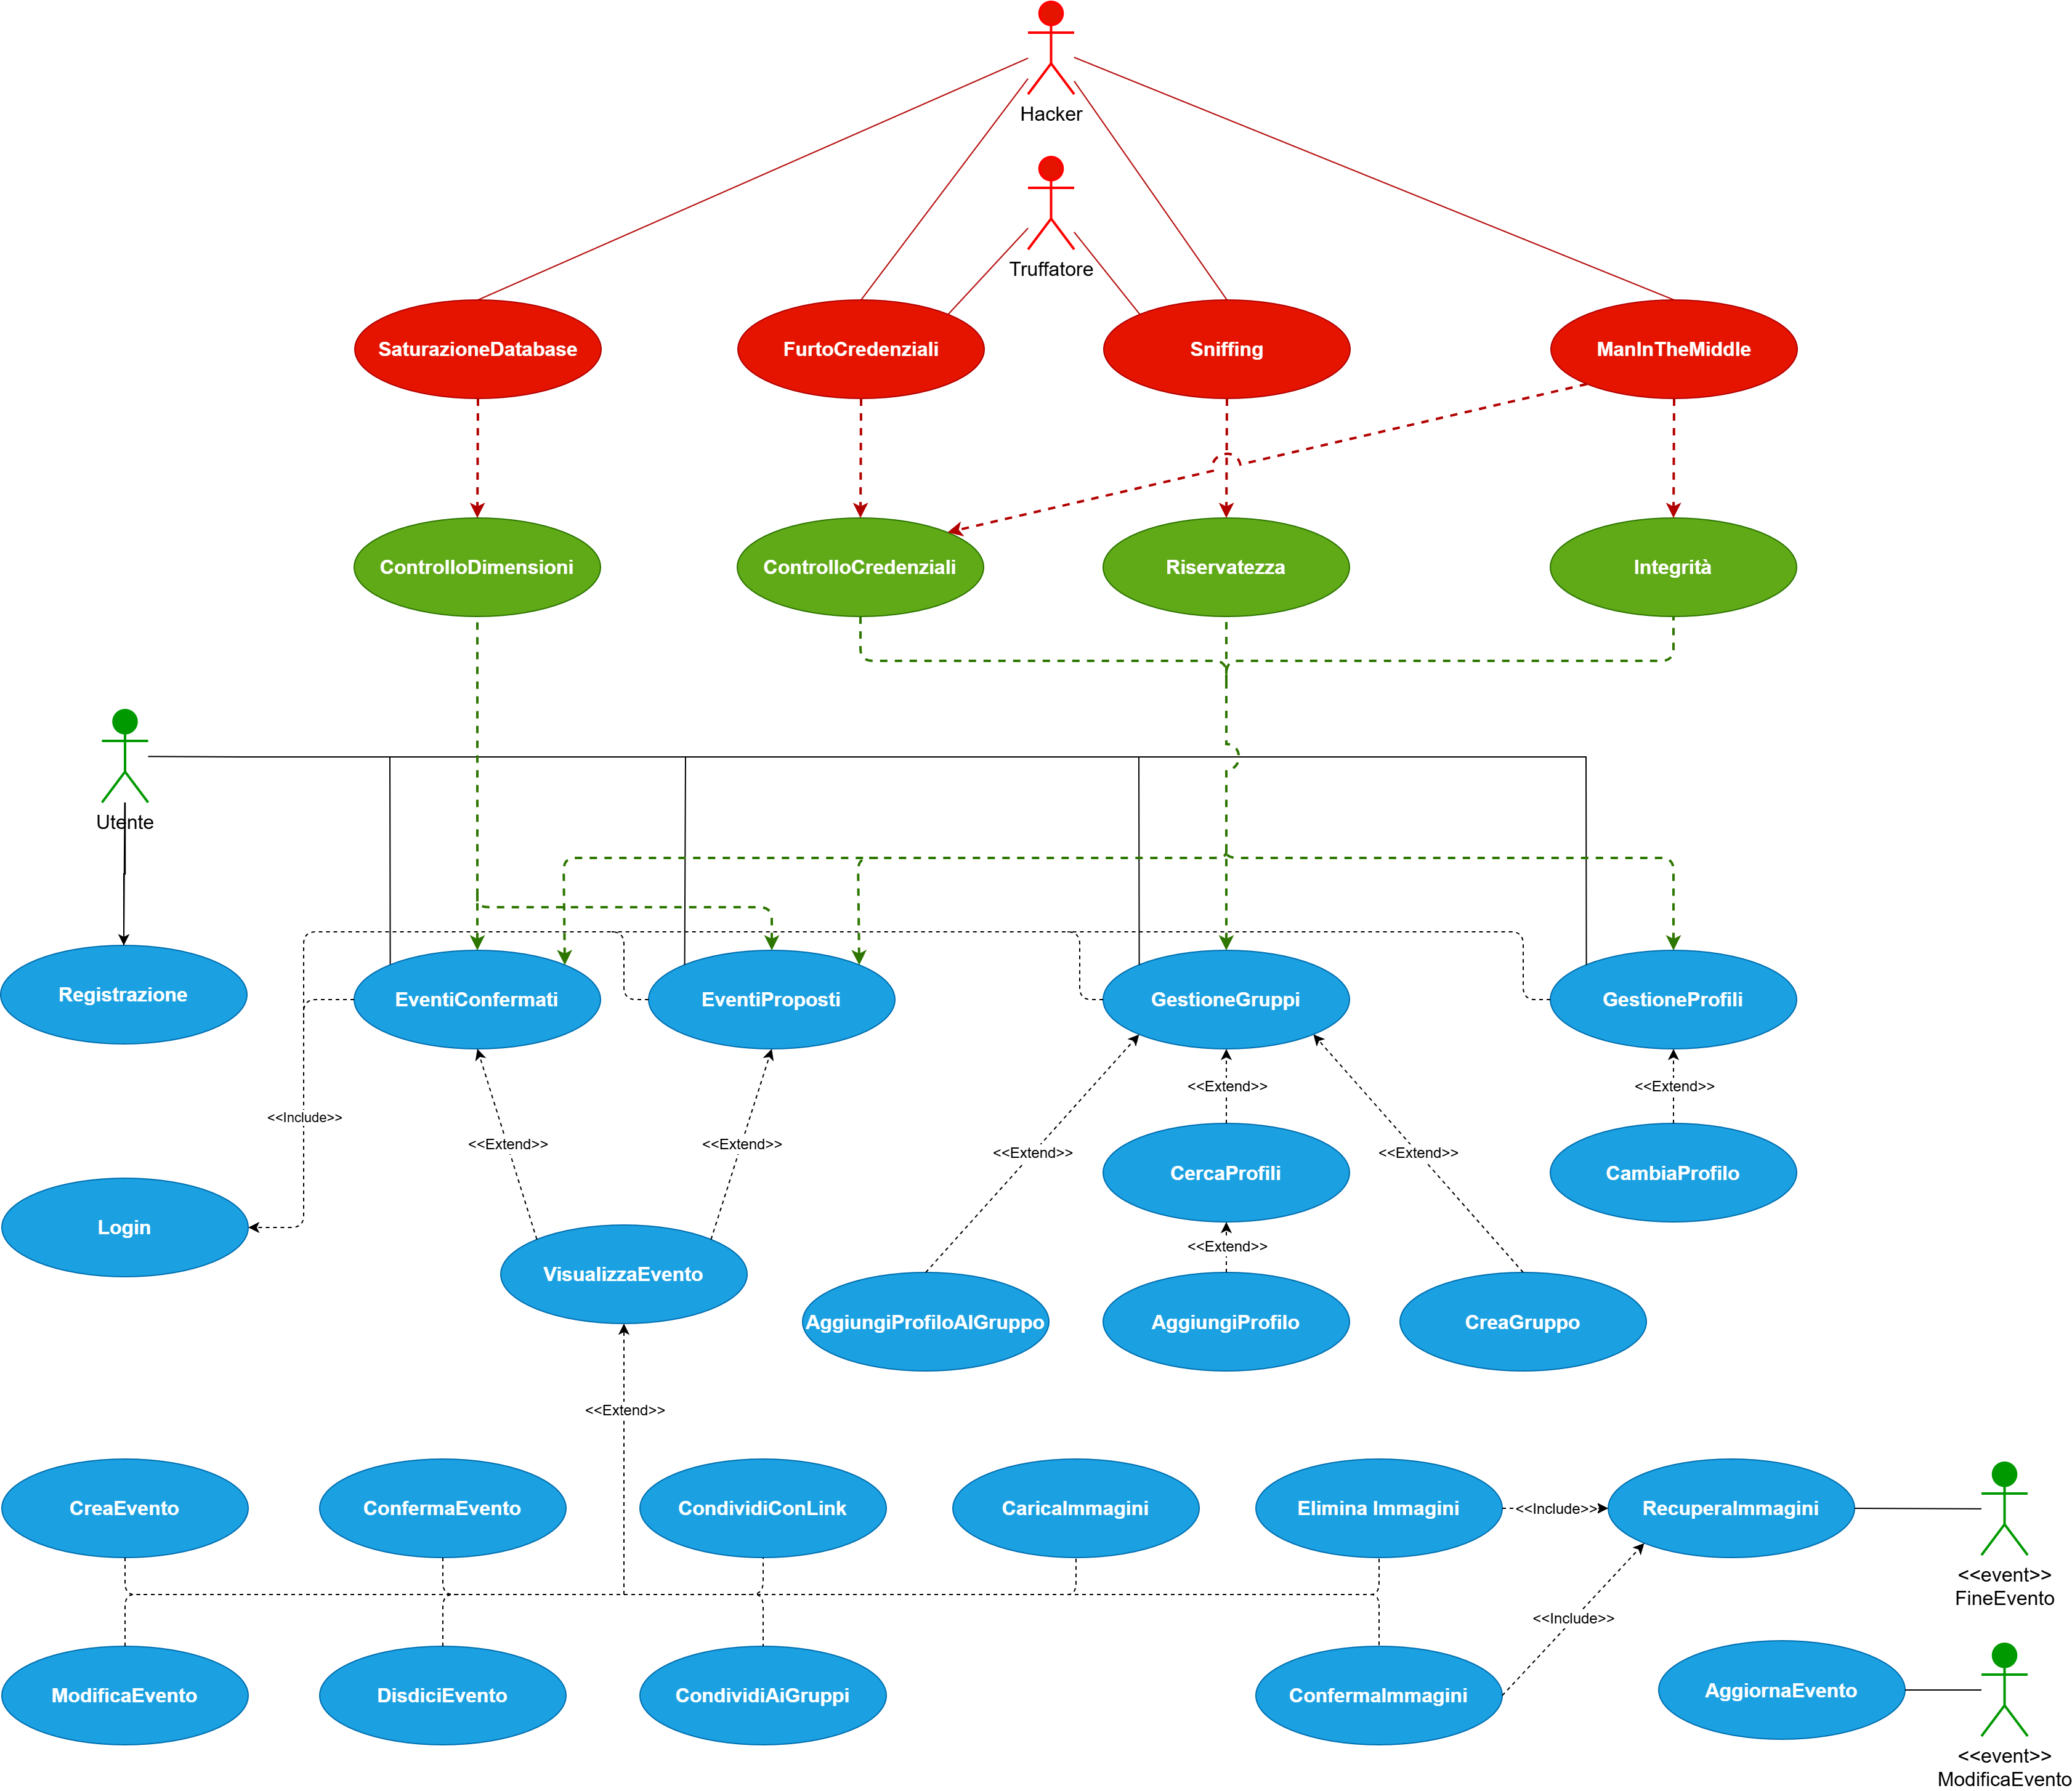
\includegraphics[width=\textwidth]{SecurityCase.png}
  \end{center}
\end{figure}
\newpage


\subsubsection{Security Use Case \& Misuse Case Scenari}
\hfill

%ControlloDimensioni
\begin{tabular} {|P{4cm}|P{11.5cm}|}
  \hline
  \textbf{Titolo}                                      & ControlloDimensioni                                                                          \\
  \hline
  \textbf{Descrizione}                                 & Le richieste non possono superare un una determinata dimensione                              \\
  \hline
  \textbf{Misuse case}                                 & SaturazioneDatabase                                                                          \\
  \hline
  \textbf{Relazioni}                                   &                                                                                              \\
  \hline
  \textbf{Precondizioni}                               & L'attaccante ha i mezzi per carpire grandi quantità di file                                  \\
  \hline
  \textbf{Postcondizioni}                              & Il sistema blocca la richiesta e limita la dimensione totale dei file caricati               \\
  \hline
  \textbf{Scenario principale}                         & 1. L'attaccante fa una richiesta con dimensioni molto grandi \linebreak
  2. Il sistema controlla le dimensioni della richiesta, e la blocca                                                                                  \\
  \hline
  \textbf{Scenari alternativi}                         & 1. L'attaccante fa tante richieste di salvataggio dati in un breve lasso di tempo \linebreak
  2. Il sistema controlla le dimensioni totali delle richieste per ogni lasso di tempo\linebreak
  3. Se le dimensioni totali superano il limite, ogni richiesta sucessiva viene bloccata fino allo scadere del tempo                                  \\
  \hline
  \textbf{Scenari di un attacco avvenuto con successo} & 1. L'attaccante riesce a farsi accettare le richieste con dimensioni elevate \linebreak
  2. Il sistema controlla la quantità totale di dati caricati dall'utente in un determinato lasso di tempo\linebreak
  3. Se la quantità supera il consentito, il sistema blocca l'utente                                                                                  \\
  \hline
\end{tabular}
\hfill
\break

%ControlloCredenziali
\begin{tabular} {|P{4cm}|P{11.5cm}|}
  \hline
  \textbf{Titolo}                                      & ControlloCredenziali                                            \\
  \hline
  \textbf{Descrizione}                                 & L'accesso alle funzionalità del sistema deve essere controllato \\
  \hline
  \textbf{Misuse case}                                 & FurtoCredenziali, ManInTheMiddle                                \\
  \hline
  \textbf{Relazioni}                                   &                                                                 \\
  \hline
  \textbf{Precondizioni}                               & L'attaccante ha i mezzi per carpire in tutto o in
  parte le credenziali di accesso di un utente                                                                           \\
  \hline
  \textbf{Postcondizioni}                              & Il sistema blocca l'accesso non autorizzato e
  notifica il tentativo di accesso                                                                                       \\
  \hline
  \textbf{Scenario principale}                         & 1. L'attaccante tenta di accedere al servizio
  spacciandosi per un utente legittimo, di cui conosce le credenziali solo in
  parte (ad esempio mediante attacco con dizionario) \linebreak 2. Il sistema non
  riconosce le credenziali, restituendo un errore \linebreak 3. In seguito ad un numero
  fissato di tentativi falliti, il sistema blocca temporaneamente l'accesso a
  quell'utente e notifica l'anomalia a chi di dovere                                                                     \\
  \hline
  \textbf{Scenari di un attacco avvenuto con successo} & 1. L'attaccante riesce
  a carpire le credenziali di accesso complete di un utente in un qualsiasi
  modo \linebreak 2. Il sistema riconosce la correttezza delle credenziali, e fornisce
  l'accesso al soggetto malevolo \linebreak 3. L'attaccante ha libero accesso al sistema,
  con privilegi diversi in base al tipo di utente                                                                        \\
  \hline
\end{tabular}
\hfill
\break

\begin{tabular} {|P{4cm}|P{11.5cm}|}
  \hline
  \textbf{Titolo}                                      & Riservatezza                                                    \\
  \hline
  \textbf{Descrizione}                                 & I dati non sono accessibili da chi non ne ha i permessi         \\
  \hline
  \textbf{Misuse case}                                 & Sniffing                                                        \\
  \hline
  \textbf{Relazioni}                                   &                                                                 \\
  \hline
  \textbf{Precondizioni}                               & L'attaccante ha i mezzi per intercettare i messaggi del sistema \\
  \hline
  \textbf{Postcondizioni}                              & Il sistema impedisce all'attaccante di decifrare
  (in tempi utili) i messaggi intercettati                                                                               \\
  \hline
  \textbf{Scenario principale}                         & 1. Il Sistema protegge i messaggi \linebreak
  2. L'attaccante riesce ad intercettare un messaggio \linebreak 3. L'attaccante prova
  a decifrare i messaggi, ma non riesce a trovare un modo per farlo abbastanza
  velocemente                                                                                                            \\
  \hline
  \textbf{Scenari di un attacco avvenuto con successo} & 1. Il Sistema protegge
  i messaggi \linebreak 2. L'attaccante riesce ad intercettare un messaggio \linebreak
  3. L'attaccante riesce a decifrare i messaggi e a leggerne il contenuto, ma
  solamente per una sessione di un utente                                                                                \\
  \hline
\end{tabular}
\hfill
\break

\begin{tabular} {|P{4cm}|P{11.5cm}|}
  \hline
  \textbf{Titolo}                                      & Integrità                                     \\
  \hline
  \textbf{Descrizione}                                 & Integrità dei dati del sistema                \\
  \hline
  \textbf{Misuse case}                                 & ManInTheMiddle                                \\
  \hline
  \textbf{Relazioni}                                   &                                               \\
  \hline
  \textbf{Precondizioni}                               & 1. L'attaccante ha i mezzi per intercettare i
  messaggi del sistema \linebreak 2. L'attaccante ha i mezzi per modificare i messaggi
  \linebreak 3. L'attaccante ha i mezzi per spedire il messaggio modificato al
  destinatario                                                                                         \\
  \hline
  \textbf{Postcondizioni}                              & Il sistema rileva il messaggio contraffatto   \\
  \hline
  \textbf{Scenario principale}                         & 1. Il Sistema protegge i messaggi \linebreak
  2. L'attaccante riesce ad intercettare un messaggio e lo modifica \linebreak 3. Il
  sistema si accorge del messaggio contraffatto e lo segna nei log                                     \\
  \hline
  \textbf{Scenari di un attacco avvenuto con successo} & 1. Il Sistema protegge
  i messaggi \linebreak 2. L'attaccante riesce ad intercettare un messaggio e
  lo modifica \linebreak 3. Il sistema accetta il messaggio e agisce di conseguenza,
  segnando il messaggio nei log                                                                        \\
  \hline
\end{tabular}
\hfill
\break

\clearpage
\subsubsection{Requisiti di Protezione dei Dati}

Sussistono inoltre i seguenti requisiti inerenti alla protezione dei dati:
\begin{enumerate}
  \item Implementare un sistema di log per tracciare tutti i messaggi tra i client e i server, inclusi gli accessi, le richieste di prenotazione, di conferma, di sospensione e di invio e ricezione di dati
  \item I dati salvati devono essere protetti da un attaccante che abbia accesso al sistema, prendendo misure di sicurezza fisica, eventualmente cifrando i dati
  \item I dati inviati tra le parti remote devono essere protetti, utilizzando la cifratura dei dati
  \item Tutte le azioni avvenute sul sistema devono essere tracciate
        tramite un sistema di log.
\end{enumerate}

\raggedright{La visione e l'analisi dei log verrà gestita
  con un editor di testo esterno, accessibile solo al personale
  autorizzato.}
\hfill \break

\begin{tabular} {|P{1.3cm}|P{11.2cm}|P{3cm}|}
  \hline
  \textbf{ID}                       & \textbf{Requisiti}                                                  & \textbf{Tipo} \\
  \hline
  R21F                              & Implementazione di un sistema di log per tracciare tutti i messaggi
  tra i client e i server           & Funzionale                                                                          \\
  \hline
  R22F                              & Le richieste non devono superare una certa dimensione               & Funzionale    \\
  \hline
  R7NF                              & I dati salvati devono essere protetti da un attaccante che abbia
  accesso al sistema, prendendo misure di sicurezza fisica, eventualmente
  cifrando i dati                   & Non Funzionale                                                                      \\
  \hline
  R8NF                              & I dati inviati tra le parti remote devono essere protetti,
  utilizzando la cifratura dei dati & Non Funzionale                                                                      \\
  \hline
\end{tabular}
\clearpage
\newpage
\section{Analisi del Problema}
\subsection{Analisi Documento dei Requisiti: Analisi delle Funzionalità}
\hfill \break

\textbf{Tabella delle Funzionalità}
\hfill \break

\begin{tabular} {|P{4cm}|P{4cm}|P{3.5cm}|P{4cm}|} % Qua cambiate a piacimento la larghezza
    \hline
    \textbf{Funzionalità} & \textbf{Tipo}                                                 & \textbf{Grado di complessità} & \textbf{Requisiti Collegati}                    \\
    \hline
    Login                 & Interazione esterno e lettura dati                            & semplice                      & R2F                                             \\
    \hline
    Registrazione         & Interazione esterno e memorizzazione dati                     & semplice                      & R1F                                             \\
    \hline
    EventiConfermati      & Interazione esterno e gestione dati                           & complessa                     & R4F, R8F                                        \\
    \hline
    EventiProposti        & Interazione esterno e gestione dati                           & complessa                     & R5F, R9F                                        \\
    \hline
    GestioneGruppi        & Interazione esterno e gestione dati                           & complessa                     & R13F, R14F                                      \\
    \hline
    GestioneProfili       & Interazione esterno e gestione dati                           & complessa                     & R10F, R12F                                      \\
    \hline
    VisualizzaEvento      & Interazione esterno e gestione, lettura e memorizzazione dati & complessa                     & R5F, R6F, R7F, R8F, R9F, R14F, R15F, R18F, R20F \\
    \hline
    AggiornaEvento        & Gestione dati                                                 & complessa                     & R17F                                            \\
    \hline
    RecuperaImmagini      & Lettura dati                                                  & complessa                     & R19F                                            \\
    \hline
    ScritturaLog          & Memorizzazione dati                                           & semplice                      & R21F                                            \\
    \hline
\end{tabular}

\hfill \break

\textbf{Registrazione: Tabella Informazioni/Flusso}
\hfill \break

\begin{tabular} {|P{3cm}|P{3cm}|P{3cm}|P{3cm}|P{3cm}|}
    \hline
    \textbf{Informazione} & \textbf{Tipo} & \textbf{Livello protezione/privacy} & \textbf{Input/Output} & \textbf{Vincoli}                                  \\
    Email                 & semplice      & Protezione alta                     & Input                 & Deve essere di 256 caratteri e del formato giusto \\
    \hline
    Password              & semplice      & Protezione molto alta               & Input                 & Deve essere almeno di 8 caratteri                 \\
    \hline
\end{tabular}
\hfill \break

\textbf{Login: Tabella Informazioni/Flusso}
\hfill \break

\begin{tabular} {|P{3cm}|P{3cm}|P{3cm}|P{3cm}|P{3cm}|}
    \hline
    \textbf{Informazione} & \textbf{Tipo} & \textbf{Livello protezione/privacy} & \textbf{Input/Output} & \textbf{Vincoli}         \\
    \hline
    Email                 & semplice      & Protezione molto alta               & Input                 & Non più di 256 caratteri \\
    \hline
    Password              & semplice      & Protezione molto alta               & Input                 & Non più di 50 caratteri  \\
    \hline
\end{tabular}
\hfill \break

\textbf{EventiConfermati: Tabella Informazioni/Flusso}
\hfill \break

\begin{tabular} {|P{3cm}|P{3cm}|P{3cm}|P{3cm}|P{3cm}|}
    \hline
    \textbf{Informazione}   & \textbf{Tipo} & \textbf{Livello protezione/privacy} & \textbf{Input / Output} & \textbf{Vincoli} \\
    \hline
    Lista Eventi Confermati & Composto      & Protezione media                    & Output                  &                  \\
    \hline
\end{tabular}
\hfill \break

\textbf{EventiProposti: Tabella Informazioni/Flusso}
\hfill \break

\begin{tabular} {|P{3cm}|P{3cm}|P{3cm}|P{3cm}|P{3cm}|}
    \hline
    \textbf{Informazione} & \textbf{Tipo} & \textbf{Livello protezione/privacy} & \textbf{Input / Output} & \textbf{Vincoli} \\
    \hline
    Lista Eventi Proposti & Composto      & Protezione media                    & Output                  &                  \\
    \hline
\end{tabular}
\hfill \break

\textbf{GestioneGruppi: Tabella Informazioni/Flusso}
\hfill \break

\begin{tabular} {|P{3cm}|P{3cm}|P{3cm}|P{3cm}|P{3cm}|}
    \hline
    \textbf{Informazione}           & \textbf{Tipo} & \textbf{Livello protezione/privacy} & \textbf{Input / Output} & \textbf{Vincoli}     \\
    \hline
    Lista Gruppi                    & Composto      & Protezione media                    & Output                  &                      \\
    \hline
    Tag di ricerca                  & Semplice      & Protezione bassa                    & Input                   &                      \\
    \hline
    Lista Profili                   & Composto      & Protezione bassa                    & Output                  & Non più di 5 profili \\
    \hline
    Identificativo Profilo corrente & Semplice      & Protezione alta                     & Output                  &                      \\
    \hline
\end{tabular}
\hfill \break

\textbf{GestioneProfili: Tabella Informazioni/Flusso}
\hfill \break

\begin{tabular} {|P{3cm}|P{3cm}|P{3cm}|P{3cm}|P{3cm}|}
    \hline
    \textbf{Informazione}           & \textbf{Tipo} & \textbf{Livello protezione/privacy} & \textbf{Input/Output} & \textbf{Vincoli} \\
    \hline
    Lista Profili                   & Composta      & Protezione media                    & Output                &                  \\
    \hline
    Identificativo Utente           & Semplice      & Protezione alta                     & Output                &                  \\
    \hline
    Identificativo Profilo corrente & Semplice      & Protezione alta                     & Output                &                  \\
    \hline
\end{tabular}
\hfill \break
\newpage
\textbf{VisualizzaEvento: Tabella Informazioni/Flusso}
\hfill \break

\begin{tabular} {|P{3cm}|P{3cm}|P{3cm}|P{3cm}|P{3cm}|}
    \hline
    \textbf{Informazione}   & \textbf{Tipo} & \textbf{Livello protezione/privacy} & \textbf{Input/Output} & \textbf{Vincoli}                          \\
    \hline
    Identificativo Evento   & Semplice      & Protezione alta                     & Output                &                                           \\
    \hline
    Titolo                  & Semplice      & Protezione media                    & Input/Output          & Non più di 256 caratteri                  \\
    \hline
    Descrizione             & Semplice      & Protezione media                    & Input/Output          & Non più di 1024 caratteri                 \\
    \hline
    Data e orario di inizio & Semplice      & Protezione media                    & Input/Output          & Deve essere precedente alla data di fine  \\
    \hline
    Data e orario di fine   & Semplice      & Protezione media                    & Input/Output          & Deve essere sucessiva alla data di inizio \\
    \hline
    Confermato              & Semplice      & Protezione media                    & Input/Output          &                                           \\
    \hline
    Immagini                & Composto      & Protezione media                    & Input/Output          &                                           \\
    \hline
    Profili associati       & Composto      & Protezione media                    & Output                &                                           \\
    \hline
\end{tabular}
\hfill \break

\textbf{AggiornaEvento: Tabella Informazioni/Flusso}
\hfill \break

\begin{tabular} {|P{3cm}|P{3cm}|P{3cm}|P{3cm}|P{3cm}|}
    \hline
    \textbf{Informazione}   & \textbf{Tipo} & \textbf{Livello protezione/privacy} & \textbf{Input/Output} & \textbf{Vincoli}                          \\
    \hline
    Identificativo Evento   & Semplice      & Protezione alta                     & Output                &                                           \\
    \hline
    Titolo                  & Semplice      & Protezione media                    & Input/Output          & Non più di 256 caratteri                  \\
    \hline
    Descrizione             & Semplice      & Protezione media                    & Input/Output          & Non più di 1024 caratteri                 \\
    \hline
    Data e orario di inizio & Semplice      & Protezione media                    & Input/Output          & Deve essere precedente alla data di fine  \\
    \hline
    Data e orario di fine   & Semplice      & Protezione media                    & Input/Output          & Deve essere sucessiva alla data di inizio \\
    \hline
    Confermato              & Semplice      & Protezione media                    & Input/Output          &                                           \\
    \hline
    Immagini                & Composto      & Protezione media                    & Input/Output          &                                           \\
    \hline
\end{tabular}
\hfill \break

\textbf{RecuperaImmagini: Tabella Informazioni/Flusso}
\hfill \break

\begin{tabular} {|P{3cm}|P{3cm}|P{3cm}|P{3cm}|P{3cm}|}
    \hline
    \textbf{Informazione} & \textbf{Tipo} & \textbf{Livello protezione/privacy} & \textbf{Input/Output} & \textbf{Vincoli} \\
    \hline
    Immagini              & Composto      & Protezione media                    & Input/Output          &                  \\
    \hline
\end{tabular}
\hfill \break

\textbf{ScritturaLog: Tabella Informazioni/Flusso}
\hfill \break

\begin{tabular} {|P{3cm}|P{3cm}|P{3cm}|P{3cm}|P{3cm}|}
    \hline
    \textbf{Informazione}  & \textbf{Tipo} & \textbf{Livello protezione/privacy} & \textbf{Input/Output} & \textbf{Vincoli}        \\
    \hline
    Data                   & semplice      & Protezione media                    & Input                 & Non più di 40 caratteri \\
    \hline
    Ora                    & semplice      & Protezione media                    & Input                 & Non più di 40 caratteri \\
    \hline
    Attore                 & semplice      & Protezione alta                     & Input                 & Non più di 20 caratteri \\
    \hline
    Identificativo Profilo & semplice      & Protezione alta                     & Input                 & Non più di 20 caratteri \\
    \hline
    Identificativo Utente  & semplice      & Protezione alta                     & Input                 & Non più di 20 caratteri \\
    \hline
    Operazione Eseguita    & composto      & Protezione alta                     & Input                 &                         \\
    \hline
    Azione                 & composto      & Protezione molto alta               & Input                 &                         \\
    \hline
\end{tabular}

\newpage
\subsubsection{Analisi Documento dei Requisiti: Analisi dei Vincoli}
\hfill \break

\textbf{Tabella Vincoli}
\hfill \break


\begin{tabular} {|P{4cm}|P{2.5cm}|P{3.5cm}|P{5.5cm}|}
    \hline
    \textbf{Requisito}                  & \textbf{Categorie} & \textbf{Impatto}                                                         & \textbf{Funzionalità} \\
    \hline
    Semplicità dell'interfaccia         & Usabilità          & Intuitività di utilizzo                                                  & TODO                  \\
    \hline
    Velocità della ricerca dei dati     & Tempo di Risposta  & Maggiore reattività                                                      &                       \\
    \hline
    Velocità di memorizzazione dei dati & Tempo di Risposta  & Maggiore reattività                                                      &                       \\
    \hline
    Controllo Accessi                   & Sicurezza          & Peggiorano tempo di risposta e usabilità, migliorano la privacy dei dati &                       \\
    \hline
    Protezione dei Dati                 & Sicurezza          & Peggiorano tempo di risposta, migliorano la privacy dei dati             &                       \\
    \hline
\end{tabular}

\newpage

\subsubsection{Analisi Documento dei Requisiti: Analisi delle Interazioni}
\hfill \break

\textbf{Tabella Maschere}
\hfill \break

\begin{tabular} {|P{5cm}|P{7cm}|P{4cm}|}
    \hline
    \textbf{Maschera}     & \textbf{Informazioni}                                                                                                              & \textbf{Funzionalità}              \\
    \hline
    View Login            & email, password                                                                                                                    & Login                              \\
    \hline
    View Registrazione    & email, password                                                                                                                    & Registrazione                      \\
    \hline
    View EventiConfermati & lista eventi confermati                                                                                                            & EventiConfermati, AggiornaEvento   \\
    \hline
    View EventiProposti   & lista eventi proposti                                                                                                              & EventiProposti, AggiornaEvento     \\
    \hline
    View VisualizzaEvento & Identificativo utente, titolo, descrizione, data e orario di inizio, data e orario di fine, confermato immagini, profili associati & VisualizzaEvento, RecuperaImmagini \\
    \hline
    View GestioneGruppi   & lista gruppi                                                                                                                       & GestioneGruppi                     \\
    \hline
    View CercaProfili     & tag di ricerca, lista profili                                                                                                      & CercaProfili                       \\
    \hline
    View GestioneProfili  & Lista profili, Identificativo utente, Identificativo profilo corrente                                                              & GestioneProfili                    \\
    \hline
\end{tabular}
\hfill \break

\textbf{Tabella Sistemi Esterni}
\hfill \break

\begin{tabular} {|P{2.5cm}|P{4cm}|P{4.5cm}|P{4.5cm}|}
    \hline
    \textbf{Sistema} & \textbf{Descrizione} & \textbf{Protocollo di Interazione} & \textbf{Livello di Sicurezza} \\
    \hline
                     &                      &                                    &                               \\
    \hline
\end{tabular}
\hfill \break

\newpage
\subsubsection{Analisi Ruoli e Responsabilità}
\hfill \break

\textbf{Tabella Ruoli}
\hfill \break

\begin{tabular} {|P{2.5cm}|P{3cm}|P{4cm}|P{3cm}|P{2.5cm}|}
    \hline
    \textbf{Ruolo} & \textbf{Responsabilità}                                                                       & \textbf{Maschere}                                                                                                                                               & \textbf{Riservatezza}                     & \textbf{Numerosità} \\
    \hline
    Utente         & Gestione di tutte le informazioni relative all'utente e ai profili, eventi e gruppi collegati & View Login, View Registrazione, View EventiConfermati, View EventiProposti, view VisualizzaEvento, View GestioneGruppi, View CercaProfili, View GestioneProfili & È richiesto un alto grado di riservatezza & Illimitati          \\
    \hline
\end{tabular}
\hfill \break


\textbf{Utente: Tabella Ruolo-Informazioni}
\hfill \break

\begin{tabular} {|P{7cm}|P{7cm}|}
    \hline
    \textbf{Informazione}   & \textbf{Tipo di Accesso} \\
    \hline
    Email                   & Lettura/Scrittura        \\
    \hline
    Password                & Lettura/Scrittura        \\
    \hline
    Lista Eventi confermati & Lettura                  \\
    \hline
    Lista Eventi Proposti   & Lettura                  \\
    \hline
    Lista Gruppi            & Lettura                  \\
    \hline
    Tag di ricerca          & Scrittura                \\
    \hline
    Lista Profili           & Lettura                  \\
    \hline
    Titolo                  & Lettura/Scrittura        \\
    \hline
    Descrizione             & Lettura/Scrittura        \\
    \hline
    Data e orario di inizio & Lettura/Scrittura        \\
    \hline
    Data e orario di fine   & Lettura/Scrittura        \\
    \hline
    Confermato              & Lettura/Scrittura        \\
    \hline
    Immagini                & Lettura/Scrittura        \\
    \hline
    Profili Associati       & Lettura                  \\
    \hline
\end{tabular}
\hfill \break
\hfill \break
\newpage

\subsubsection{Scomposizione del Problema}
\hfill \break

\textbf{Tabella Scomposizione Funzionalità}
\hfill \break

\begin{tabular} {|P{7cm}|P{7cm}|}
    \hline
    \textbf{Funzionalità} & \textbf{Scomposizione}                                                                                                                            \\
    \hline
    EventiConfermati      & VisualizzaEvento                                                                                                                                  \\
    \hline
    EventiProposti        & VisualizzaEvento                                                                                                                                  \\
    \hline
    VisualizzaEvento      & CreaEvento, ModificaEvento, ConfermaEvento, DisdiciEvento, CondividiConLink, CondividiAiGruppi, CaricaImmagini, EliminaImmagini, ConfermaImmagini \\
    \hline
    GestioneGruppi        & CercaProfili, AggiungiProfiloAlGruppo, CreaGruppo                                                                                                 \\
    \hline
    CercaProfili          & AggiungiProfilo                                                                                                                                   \\
    \hline
    GestioneProfili       & CambiaProfilo                                                                                                                                     \\
    \hline
\end{tabular}
\hfill \break

Non sono presenti legami di esclusione o di necessità tra le sotto-funzionalità del sistema.

\newpage
\subsubsection{Creazione Modello del Dominio}

Il seguente diagramma delle classi rappresenta la parte di modello del dominio relativa al sistema. \\

\begin{figure}[h!]
    \begin{center}
        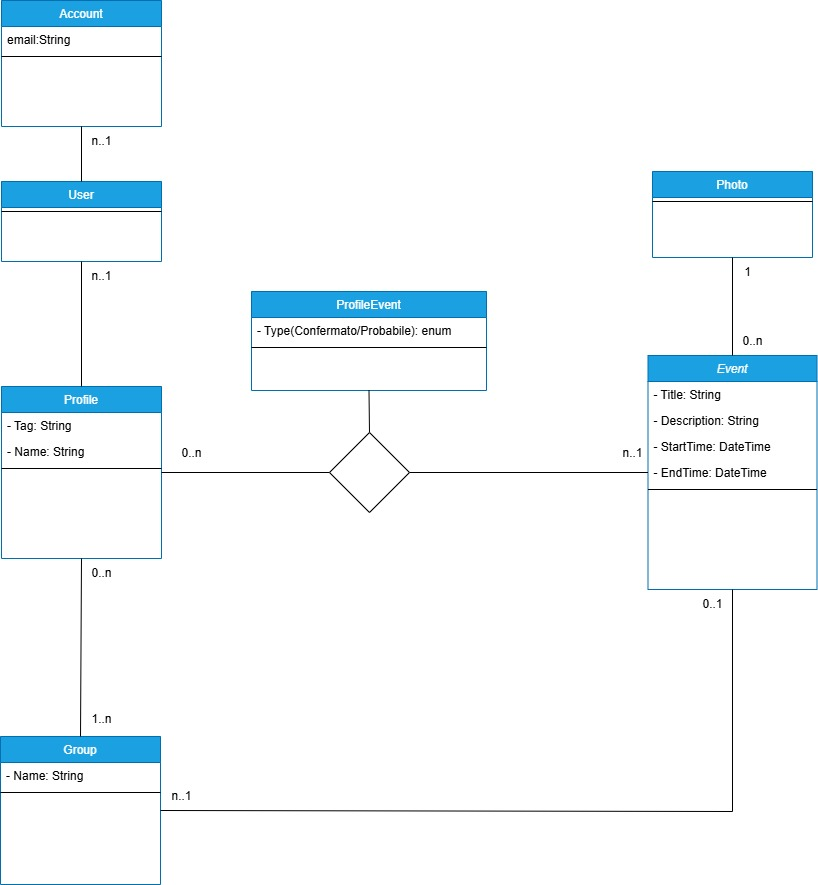
\includegraphics[width=\textwidth]{ModelloDominio.jpg}
    \end{center}
\end{figure}
\hfill \break

\newpage
\subsubsection{Architettura Logica: Struttura}
\hfill \break

\textbf{Diagramma dei package}
\hfill \break

\begin{figure}[h!]
    \begin{center}
        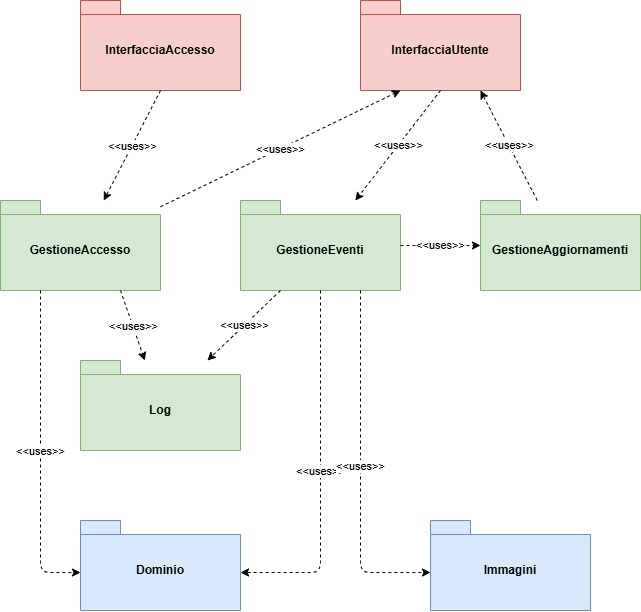
\includegraphics[width=\textwidth]{DiagrammaPackage.jpg}
    \end{center}
\end{figure}
\hfill \break

\textbf{Diagramma delle classi: Dominio}
\hfill \break

Non viene riportato il diagramma delle classi associato al package Dominio in quanto è il modello del dominio creato nella fase precedente.

\newpage

\textbf{Diagramma delle classi: InterfacciaAccesso \& GestioneAccesso}
\hfill \break

\begin{figure}[h!]
    \begin{center}
        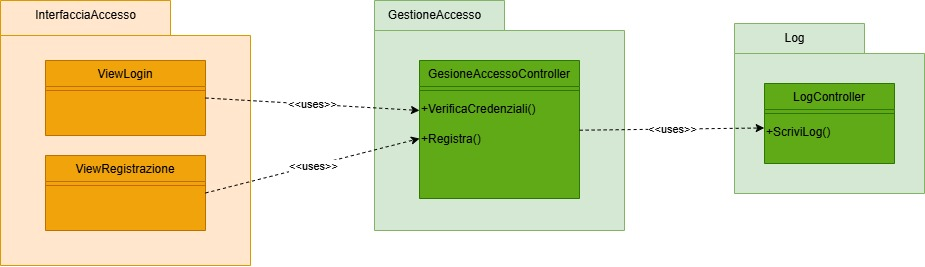
\includegraphics[width=\textwidth]{GestioneAccesso.jpg}
    \end{center}
\end{figure}
\hfill \break

\textbf{Diagramma delle classi: InterfacciaUtente \& GestioneProfilo \& GestioneAggiornamenti }

\begin{figure}[h!]
    \begin{center}
        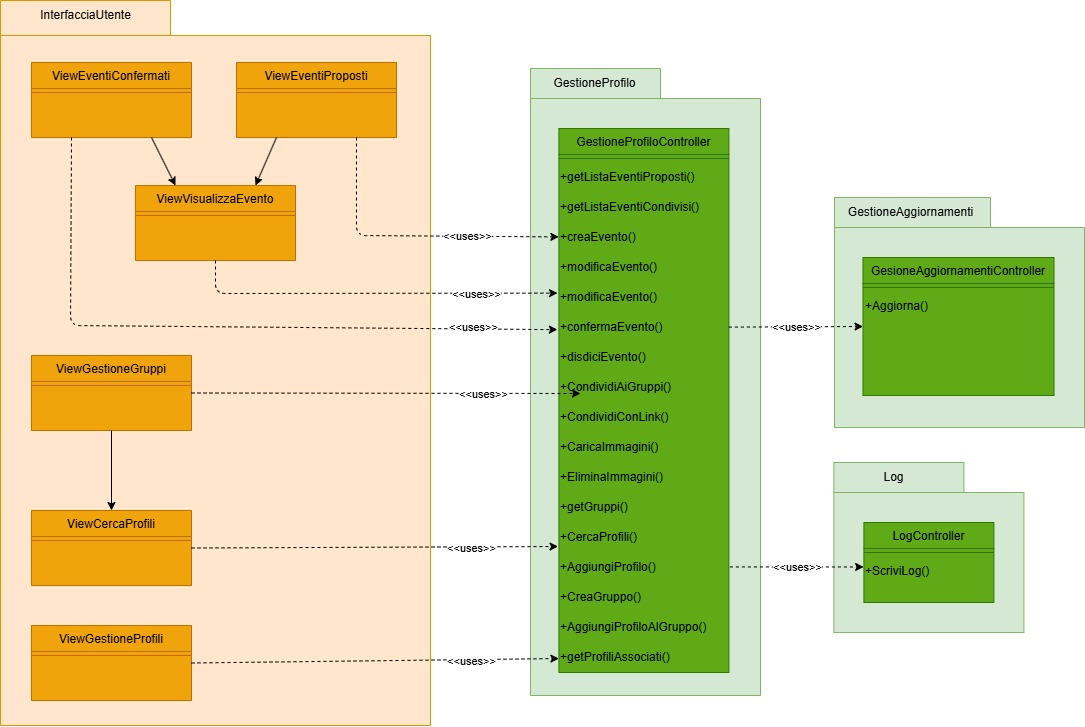
\includegraphics[width=\textwidth]{GestioneProfilo.jpg}
    \end{center}
\end{figure}
\hfill \break
\newpage

\subsubsection{Architettura Logica: Interazione}

In seguito saranno riportati i principali diagrammi di sequenza durante un normale utilizzo dell'applicazione.
\hfill \break

\textbf{Diagramma di Sequenza: Login Utente}

\begin{figure}[h!]
    \begin{center}
        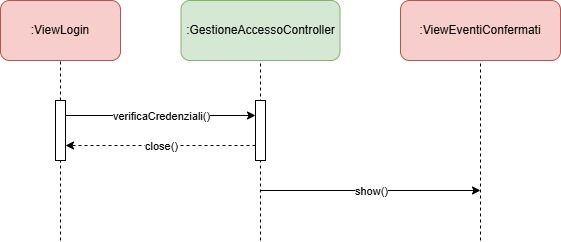
\includegraphics[scale=0.8]{SequenzaLogin.jpg}
    \end{center}
\end{figure}
\hfill \break

\textbf{Diagramma di Sequenza: Registrazione}

\begin{figure}[h!]
    \begin{center}
        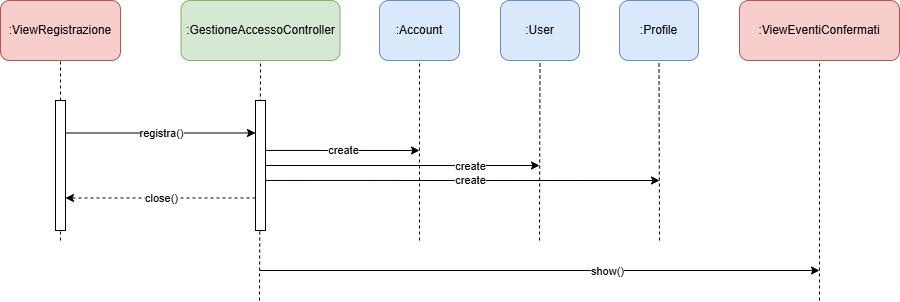
\includegraphics[width=\textwidth]{SequenzaRegistrazione.jpg}
    \end{center}
\end{figure}
\hfill \break
\newpage

\textbf{Diagramma di Sequenza: Visualizza Eventi Confermati}

\begin{figure}[h!]
    \begin{center}
        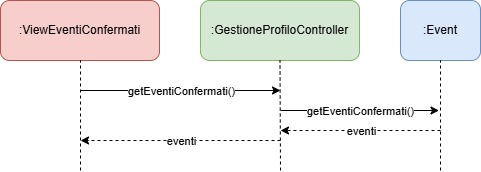
\includegraphics[scale=0.8]{SequenzaVisualizzaEventiConfermati.jpg}
    \end{center}
\end{figure}
\hfill \break

\textbf{Diagramma di Sequenza: Visualizza Eventi Proposti}

\begin{figure}[h!]
    \begin{center}
        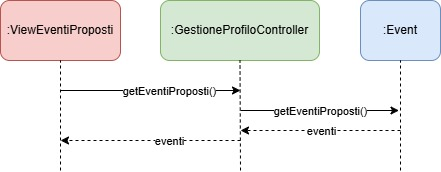
\includegraphics[scale=0.8]{SequenzaVisualizzaEventiProposti.jpg}
    \end{center}
\end{figure}
\hfill \break
\newpage
\textbf{Diagramma di Sequenza: Visualizza Evento}

\begin{figure}[h!]
    \begin{center}
        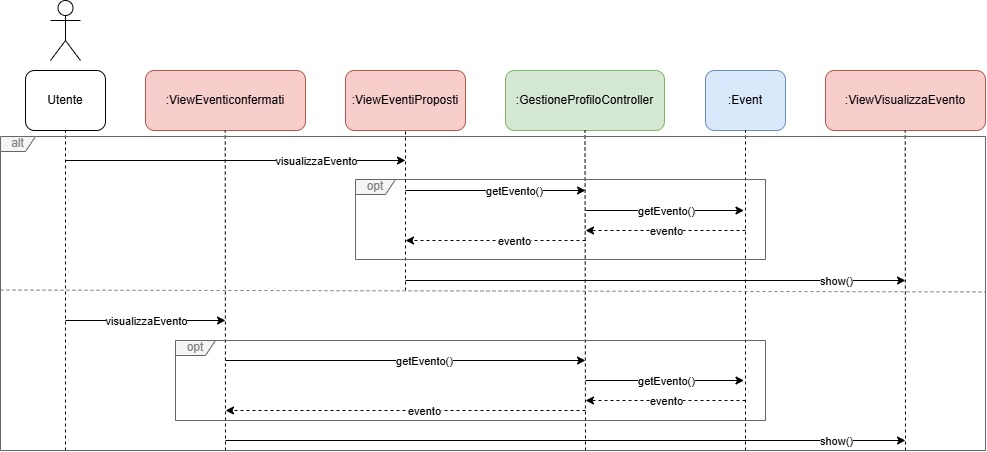
\includegraphics[width=\textwidth]{SequenzaVisualizzaEvento.jpg}
    \end{center}
\end{figure}
\hfill \break


\textbf{Diagramma di Sequenza: Crea / Modifica / Conferma / Disdici Evento}

\begin{figure}[h!]
    \begin{center}
        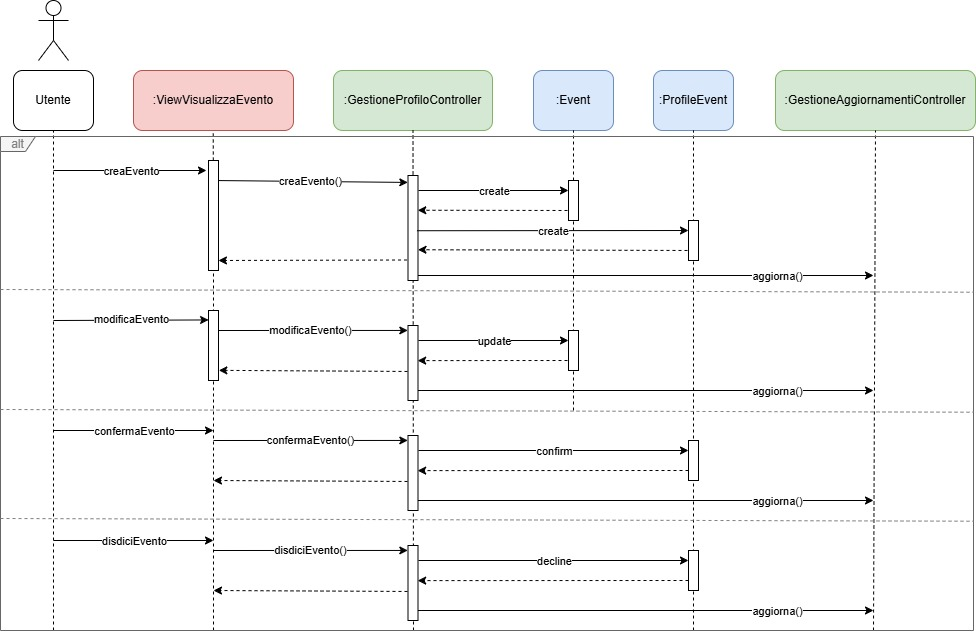
\includegraphics[width=\textwidth]{SequenzaCreaModificaEvento.jpg}
    \end{center}
\end{figure}
\hfill \break

\textbf{Diagramma di Sequenza: Carica Immagini}

\begin{figure}[h!]
    \begin{center}
        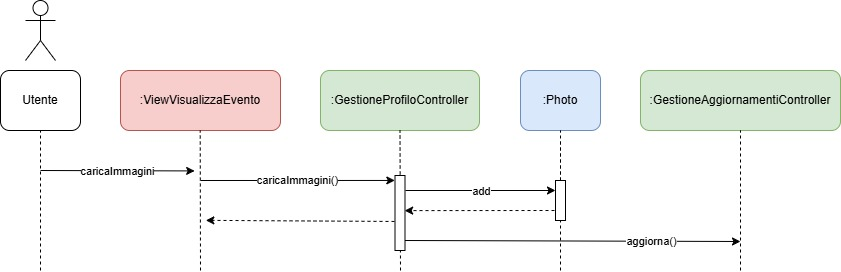
\includegraphics[width=\textwidth]{SequenzaCaricaImmagini.jpg}
    \end{center}
\end{figure}
\hfill \break

\textbf{Diagramma di Sequenza: Conferma Immagini}

\begin{figure}[h!]
    \begin{center}
        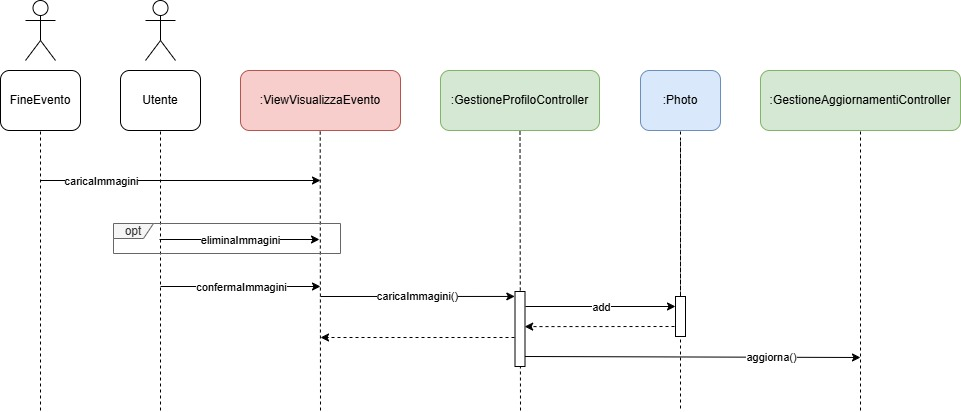
\includegraphics[width=\textwidth]{SequenzaConfermaImmagini.jpg}
    \end{center}
\end{figure}
\hfill \break
\newpage

\textbf{Diagramma di Sequenza: Condividi Evento ai gruppi}

\begin{figure}[h!]
    \begin{center}
        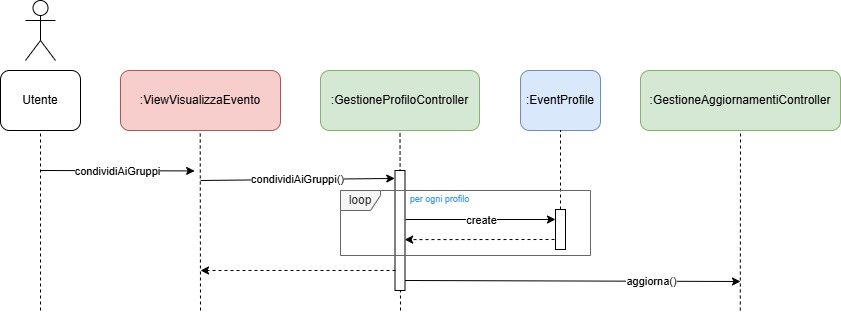
\includegraphics[width=\textwidth]{SequenzaCondividiEvento.jpg}
    \end{center}
\end{figure}
\hfill \break

\newpage
\subsubsection{Piano di Lavoro}

I compiti sono stati divisi in base alle competenze di
ogni membro del gruppo come indicato nella tabella sottostante:
\hfill \break

\begin{tabular} {|P{5cm}|P{5cm}|P{5cm}|} % Qua cambiate a piacimento la larghezza
    \hline
    \textbf{Package}      & \textbf{Progetto} & \textbf{Sviluppo} \\
    \hline
    GestioneAccesso       & Romanini          & Romanini          \\
    \hline
    GestioneEventi        & Romanini          & Romanini          \\
    \hline
    GestioneAggiornamenti & Romanini          & Romanini          \\
    \hline
    InterfacciaUtente     & Romanini          & Romanini          \\
    \hline
    InterfacciaAccesso    & Romanini          & Romanini          \\
    \hline
    Dominio               & Romanini          & Romanini          \\
    \hline
    Immagini              & Romanini          & Romanini          \\
    \hline
    Log                   & Romanini          & Romanini          \\
    \hline
\end{tabular}
\hfill \break

I tempi di rilascio sono i seguenti:
\begin{itemize}
    \item Progettazione entro due settimane dalla data odierna
    \item Sviluppo dei vai moduli con annessi test unitari entro due mesi dalla fine della fase di progettazione
    \item Integrazione e testing del sistema entro un mese dalla fine dello sviluppo
\end{itemize}
\hfill \break

\textbf{Sviluppi Futuri}
\\

TODO
Chat tra gli utenti
Eventi pubblici
gestione biglietti per gli eventi
funzionalità aggiuntive di condivisione eventi
visualizzazione eventi degli altri profili

%\newpage
\subsubsection{Piano del Collaudo}

Per verificare il corretto funzionamento del sistema sono necessari dei test
unitari che ne verifichino la correttezza delle singole parti. In seguito
verranno riportati i casi reputati più importanti in fase di analisi.

\usemintedstyle{manni}
\begin{minted}
[
frame=lines,
framesep=2mm,
baselinestretch=1.2,
bgcolor=LightGray,
fontsize=\footnotesize,
linenos
]
{java}
public class testPrenotazione{
    private Prenotazione prenotazione;

    @Before
    public void setUp(){
       prenotazione = new Prenotazione();
    }

    @Test
    public void testCostruttore(){
        prenotazione = new Prenotazione(new SimpleDateFormat("2021-06-01"), true);
        Assert.assertNull(prenotazione.isConfermata());
    }

    @Test
    public void testGetter(){
        prenotazione = new Prenotazione(new SimpleDateFormat("2021-06-01"), true);
        Assert.assertEquals(prenotazione.getData(), new SimpleDateFormat("2021-06-01"));
        Assert.assertEquals(prenotazione.getConfermata(), true);
    }

    @Test
    public void testSetter(){
        prenotazione.setData(new SimpleDateFormat("2021-07-02"));
        Assert.assertEquals(prenotazione.getData(), new SimpleDateFormat("2021-07-02"));
        prenotazione.setConfermata(true);
        Assert.assertEquals(prenotazione.getConfermata(), true);
    }
}

public class testFarmacia{
    private Farmacia farmacia;

    @Before 
    public void setUp(){
        farmacia = new Farmacia();
    }

    @Test
    public void testCostruttore(){
        Assert.assertNull(farmacia.getNome());
        Assert.assertNull(farmacia.getId());
    }

    @Test 
    public void testGetter(){
        farmacia = new Farmacia("N23N230SD", "Ubertini", "BO", "Bologna", "via Libia", "10");
        Assert.assertEquals(farmacia.getId(),"N23N230SD");
        Assert.assertEquals(farmacia.getNome(),"Ubertini");
        Assert.assertEquals(farmacia.getProvincia(),"BO");
        Assert.assertEquals(farmacia.getComune(),"Bologna");
        Assert.assertEquals(farmacia.getVia(),"via Libia");
        Assert.assertEquals(farmacia.getNumeroCivico(),"10");
    }

    @Test 
    public void testSetter(){
        farmacia.setId("N23N230SD");
        Assert.assertEquals(farmacia.getId(),"N23N230SD");
        farmacia.setNome("Ubertini");
        Assert.assertEquals(farmacia.getNome(),"Ubertini");
        farmacia.setProvincia("BO");
        Assert.assertEquals(farmacia.getProvincia(),"BO");
        farmacia.setComune("Bologna");
        Assert.assertEquals(farmacia.getComune(),"Bologna");
        farmacia.setVia("via Libia");
        Assert.assertEquals(farmacia.getVia(),"via Libia");
        farmacia.setNumeroCivico("10");
        Assert.assertEquals(farmacia.getNumeroCivico(),"10");
    }
}

public class testCliente{
    private ClienteRegistrato cliente;

    @Before 
    public void setUp(){
        cliente = new ClienteRegistrato();
    }

    @Test 
    public void testGetter(){
        cliente = new ClienteRegistrato("Federico", "Chesani", new
        SimpleDateFormat("1920-07-10"), "CHSFRC20L10A944G",
        "federico.chesani@unibo.it", 0, null, true, false);
        Assert.assertEquals(cliente.getNome(), "Federico");
        Assert.assertEquals(cliente.getCognome(), "Chesani");
        Assert.assertEquals(cliente.getNascita(), new SimpleDateFormat("1920-07-10"));
        Assert.assertEquals(cliente.getCodiceFiscale(), "CHSFRC20L10A944G");
        Assert.assertEquals(cliente.getEmail(), "federico.chesani@unibo.it");
        Assert.assertEquals(cliente.getEffrazioni(), 0);
        Assert.assertEquals(cliente.isVerificato(), true);
        Assert.assertEquals(cliente.isBloccato(), false);
    }

    @Test 
    public void testSetter(){
        cliente.setNome("Federico");
        Assert.assertEquals(cliente.getNome(), "Federico");
        cliente.setCognome("Chesani");
        Assert.assertEquals(cliente.getCognome(), "Chesani");
        cliente.setNascita(new SimpleDateFormat("1920-07-10"));
        Assert.assertEquals(cliente.getNascita(), new SimpleDateFormat("1920-07-10"));
        cliente.setCodiceFiscale("CHSFRC20L10A944G");
        Assert.assertEquals(cliente.getCodiceFiscale(), "CHSFRC20L10A944G");
        cliente.setEmail("federico.chesani@unibo.it");
        Assert.assertEquals(cliente.getEmail(), "federico.chesani@unibo.it");
        cliente.setEffrazioni(0);
        Assert.assertEquals(cliente.getEffrazioni(), 0);
        cliente.setVerificato(true);
        Assert.assertEquals(cliente.isVerificato(), true);
        cliente.setBloccato(false);
        Assert.assertEquals(cliente.isBloccato(), false);
    }
}
\end{minted}

%\newpage
\section{Progettazione}

\subsection{Progettazione Architetturale}

\subsubsection{Requisiti non funzionali}

Dall'analisi dei requisiti sono emersi i seguenti requisiti non funzionali:
\begin{itemize}
    \item Tempo di risposta
    \item Usabilità
    \item Affidabilità
    \item Scalabilità
    \item Integrità dei dati
    \item Protezione dei dati
    \item Sicurezza delle comunicazioni
\end{itemize}

L'affidabilità e la scalabilità assumono fondamentale importanza vista la natura del software,
che deve permettere agli utenti di poter organizzare, coordinare e condividere eventi.
La compromissione di questi risulterebbe in un peggioramento dell'esperienza utente, da cui consegue una perdita di reputazione o di fedeltà del cliente.
Sarà necessario assicurare la sicurezza fisica dei dati immagazzinati nel sistema, così come la sicurezza software dei dati e delle comunicazioni.
In caso di compromissione la perdita d'immagine e i risvolti legali sarebbero significativi.
L'utilizzo di protocolli e tecnologie standard del settore dovrebbero garantire la sicurezza del sitema senza peggiorarne significativamente l'usabilità o le prestazioni.
Nonostante il sistema non presenti vincoli di tempo stringenti, una caratteristica essenziale dell'applicazione sarà la velocità di distribuire gli aggiornamenti ai vari utenti.
Inoltre, l'intuitività dell'interfaccia è fondamentale per l'usabilità e la diffusione del prodotto.

\subsubsection{Scelte tecnologiche}

La scelta tecnologica principale ricade sul tipo di applicazione che si andrà a
sviluppare.
In questo caso la scelta è quella di sviluppare sia un'applicazione sia da browser web, che tramite dispositivo mobile, per i seguenti motivi:
\begin{enumerate}
    \item un'interfaccia web consente di avere una
          piattaforma standard accessibile da quasi tutti i dispositivi, con il solo
          requisito di un browser, potenzialmente permettendo(in base alla dimensione dello schermo) una maggior facilità di utilizzo, per rispondere all'esigenza organizzativa di medio o lungo termine.
          In questo modo si evita di restringere le possibilità di accesso al servizio.
    \item  l'applicazione mobile permette una gestione a breve termine e un aggiornamento costante, ed è fondamentale per recuperare le immagini dell'utente.
\end{enumerate}
\newpage
\subsubsection{Scelta dell'architettura}

Dopo una rapida analisi, si è constatato che l'architettura più adeguata per il
sistema è l'\textbf{architettura client-server a 3 livelli}.

\paragraph{L1 -- Client}\mbox{}\\
La componente lato Client implementerà l'interfaccia utente, gestendo le interazioni del cliente e richiedendo i dati al server,
salvandoli in una cache locale laddove la tecnologia lo renda possibile. Inoltre avrà la responsabilità di recuperare le immagini scattate durante l'evento.

\paragraph{L2 -- Server}\mbox{}\\
Per distribuire meglio il carico, si è deciso di scomporre i server in base alle funzionalità offerte. Si hanno quindi tre server:

\begin{itemize}
    \item[-] Un server per le funzionalità di autenticazione
    \item[-] Un server principale che fornisce i servizi agli utenti
    \item[-] Un server che gestisce la propagazione degli aggiornamenti agli utenti
\end{itemize}

\paragraph{L3 -- Persistenza}\mbox{}\\
La gestione della persistenza verrà implementata in due server con responsabilità differenti:
\begin{itemize}
    \item[-] Un server sul quale sarà installato un DBMS che gestisca i dati e le relazioni dei componenti
    \item[-] Un server per il salvataggio delle immagini e file
\end{itemize}

Il database relazionale sarà accessibile solo dal server che fornisce i servizi, per garantire il controllo dei ruoli e dei permessi.
Le immagini saranno invece accessibili solo in lettura direttamente dai client, che dovranno però essere a conoscenza dei codici che le identificano.
Questa conoscenza è considerata sufficente per garantire la confidenza, ammesso che l'identificativo sia lungo abbastanza, 
ma anche un rischio accettabile, in quanto ridurrà di molto il carico del server principale. 

\subsubsection{Pattern architetturali e di design}

Il pattern Client-Server è stato scelto come pattern architetturale per gestire l'accesso, le immagini e i servizi principali.\\
Il pattern Event Driven sarà invece usato per notificare i Client degli aggiornamenti.
A livello di design distinguiamo tre componenti principali: Model, View e Controller.
Mentre la View sarà delegata completamente ai Client, Model e Controller saranno invece suddivisi tra il Client e il Server, 
in base alle necessità di caching dei dati e della località delle operazioni di business.\\
Si riportano di seguito i diagrammi di package e componenti che descrivono l'architettura del sistema.

\newpage

\begin{figure}[h!]
    \begin{center}
        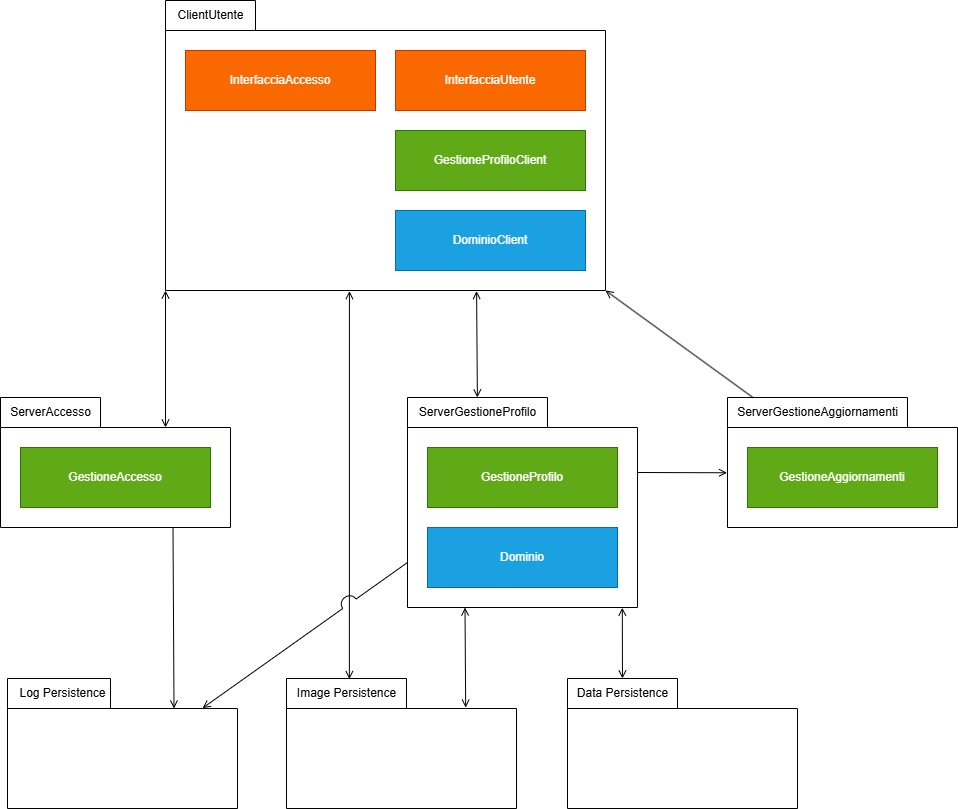
\includegraphics[width=\textwidth]{ProgettoDiagrammaPackage.jpg}
        \caption{Diagramma dei package}
    \end{center}
\end{figure}

\newpage

\begin{figure}[h!]
    \begin{center}
        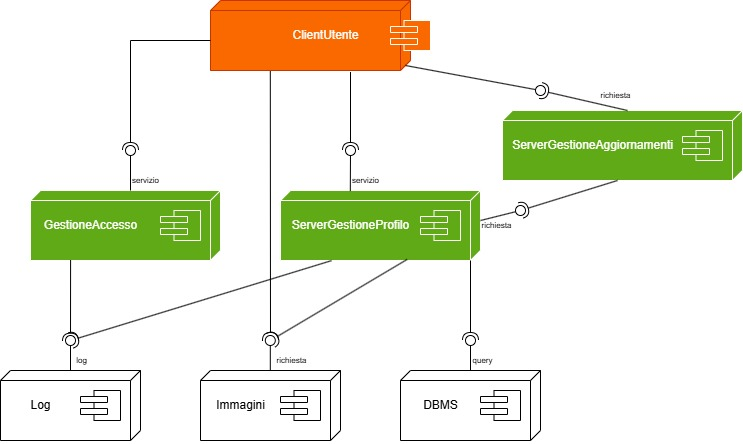
\includegraphics[width=\textwidth]{ProgettoDiagrammaComponenti.jpg}
        \caption{Diagramma dei componenti}
    \end{center}
\end{figure}

\newpage

\subsection{Progettazione di dettaglio}

\subsubsection{Struttura}

\textbf{Struttura: Dominio}\\

Per quanto riguarda il dominio, distinguiamo il dominio del server dal dominio del client.

\vspace{1em}

\textbf{Diagramma di dettaglio: Dominio Server}\\
Aggiungiamo a tutti i componenti principali un identificativo anfanumerico chiamato hash, 
e le date di creazione e di ultima modifica per gestire meglio i log e gli aggiornamenti.
Inoltre, aggiungiamo un componente per definire il ruolo dell'utente sul profilo.
\begin{figure}[h!]
    \begin{center}
        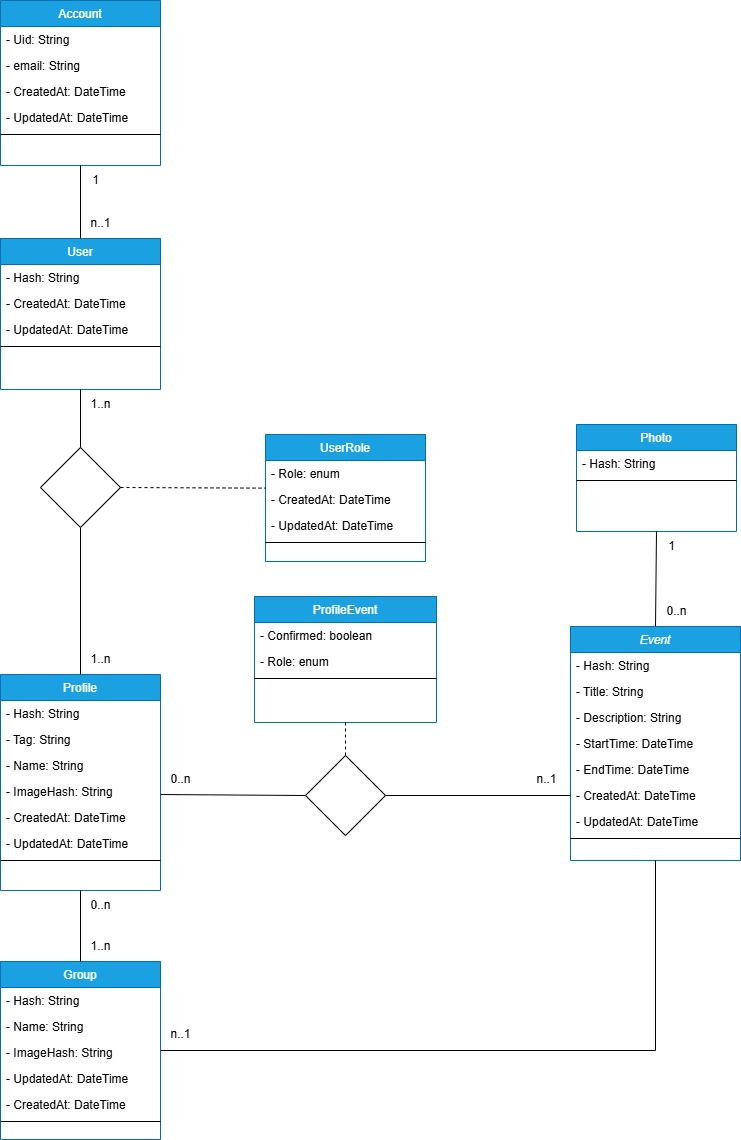
\includegraphics[scale=0.45]{ProgettoDominioServer.jpg}
    \end{center}
\end{figure}

\newpage

\textbf{Diagramma di dettaglio: Dominio Client}\\
Dal punto di vista del client alcune relazioni non sono più rilevanti o vengono semplificate integrando alcuni valori all'interno di altri elementi del dominio. 
\begin{figure}[h!]
    \begin{center}
        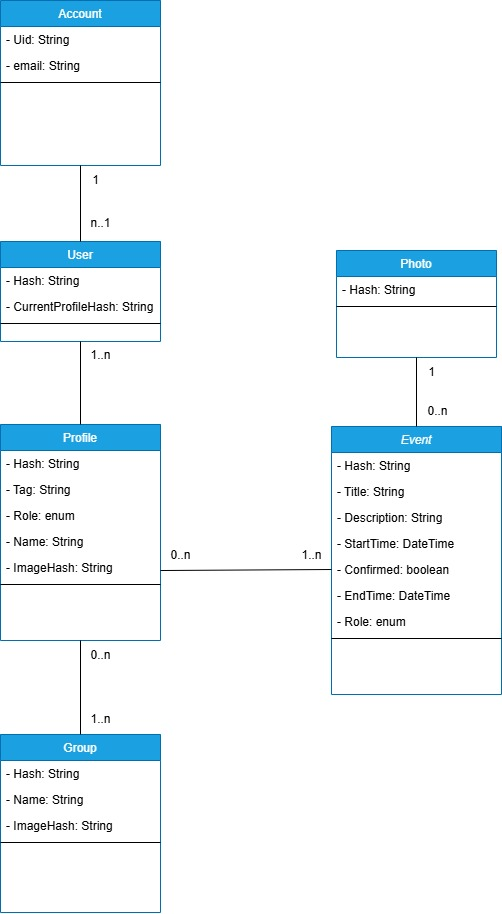
\includegraphics[scale=0.56]{ProgettoDominioClient.jpg}
    \end{center}
\end{figure}
\clearpage
\newpage

\textbf{Diagramma di dettaglio: Interfacce Gestione Accesso e Gestione Aggiornamenti}
\begin{figure}[h!]
    \begin{center}
        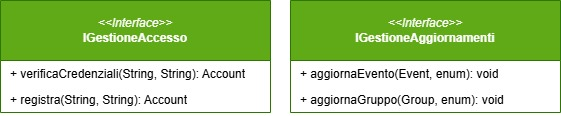
\includegraphics[width=\textwidth]{ProgettoInterfacceAccesso.jpg}
    \end{center}
\end{figure}
\\
\textbf{Diagramma di dettaglio: Interfacce Client}
\begin{figure}[h!]
    \begin{center}
        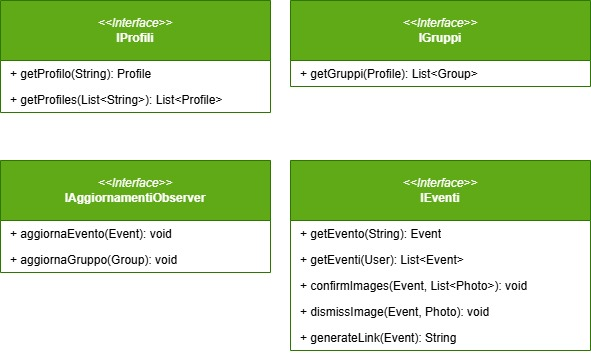
\includegraphics[width=\textwidth]{ProgettoInterfacceClient.jpg}
    \end{center}
\end{figure}
\newpage
\textbf{Diagramma di dettaglio: Interfacce Server}
\begin{figure}[h!]
    \begin{center}
        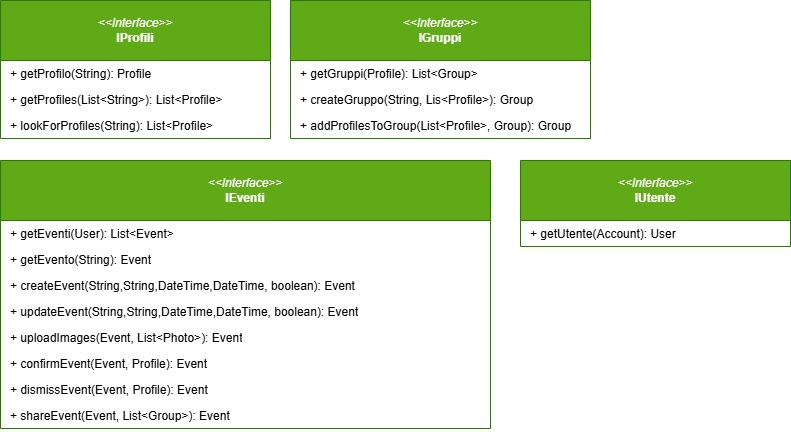
\includegraphics[width=\textwidth]{ProgettoInterfacceServer.jpg}
    \end{center}
\end{figure}\\

Le interfacce client e server risultano molto simili in quanto il client, prima di fare una richiesta dati al server, controllerà la cache locale per cercare i dati.
L'aggiunta di tali interfacce consente di applicare il \textit{Dependency Inversion Principle}
in modo da disaccoppiare gli utilizzatori dalle implementazioni, che potrebbero cambiare.


\newpage

\paragraph{Struttura: Controller}\mbox{}\\

Ogni interfaccia verrà implementata da un relativo controller.
\vspace{2em}

\textbf{Diagramma di dettaglio: Gestione Accesso e Gestione Aggiornamenti}
\\Introduciamo un Controller per la connessione con la persistenza del log
\begin{figure}[h!]
    \begin{center}
        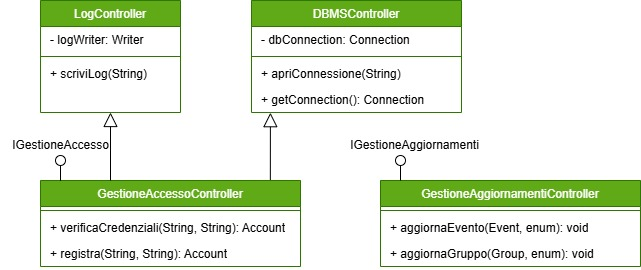
\includegraphics[width=\textwidth]{ProgettoControllerAccesso.jpg}
    \end{center}
\end{figure}

\newpage

\textbf{Diagramma di dettaglio: Client}
\begin{figure}[h!]
    \begin{center}
        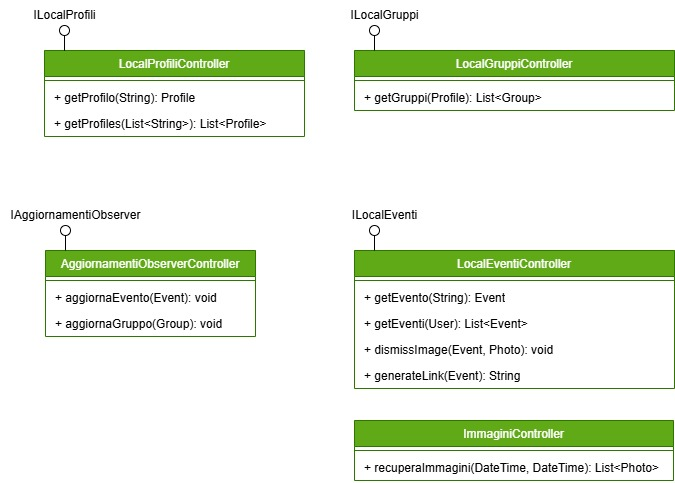
\includegraphics[width=\textwidth]{ProgettoControllerClient.jpg}
    \end{center}
\end{figure}


\newpage

\textbf{Diagramma di dettaglio: Server}
\begin{figure}[h!]
    \begin{center}
        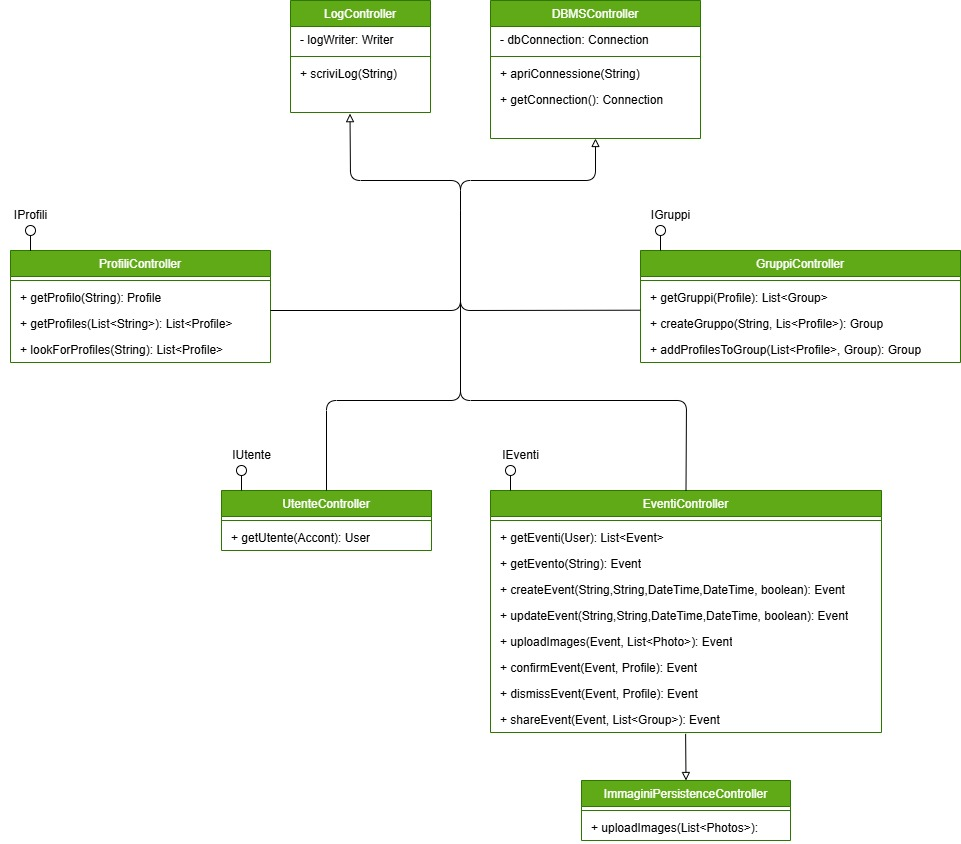
\includegraphics[width=\textwidth]{ProgettoControllerServer.jpg}
    \end{center}
\end{figure}

\newpage





\textbf{Diagramma di dettaglio: InterfacciaUtente - Eventi}
\begin{figure}[h!]
    \begin{center}
        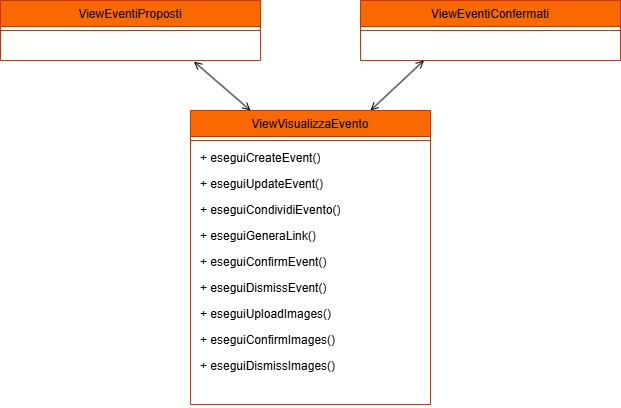
\includegraphics[width=0.9\textwidth]{ProgettoViewEventi.jpg}
    \end{center}
\end{figure}
\begin{figure}[h!]
    \centering
    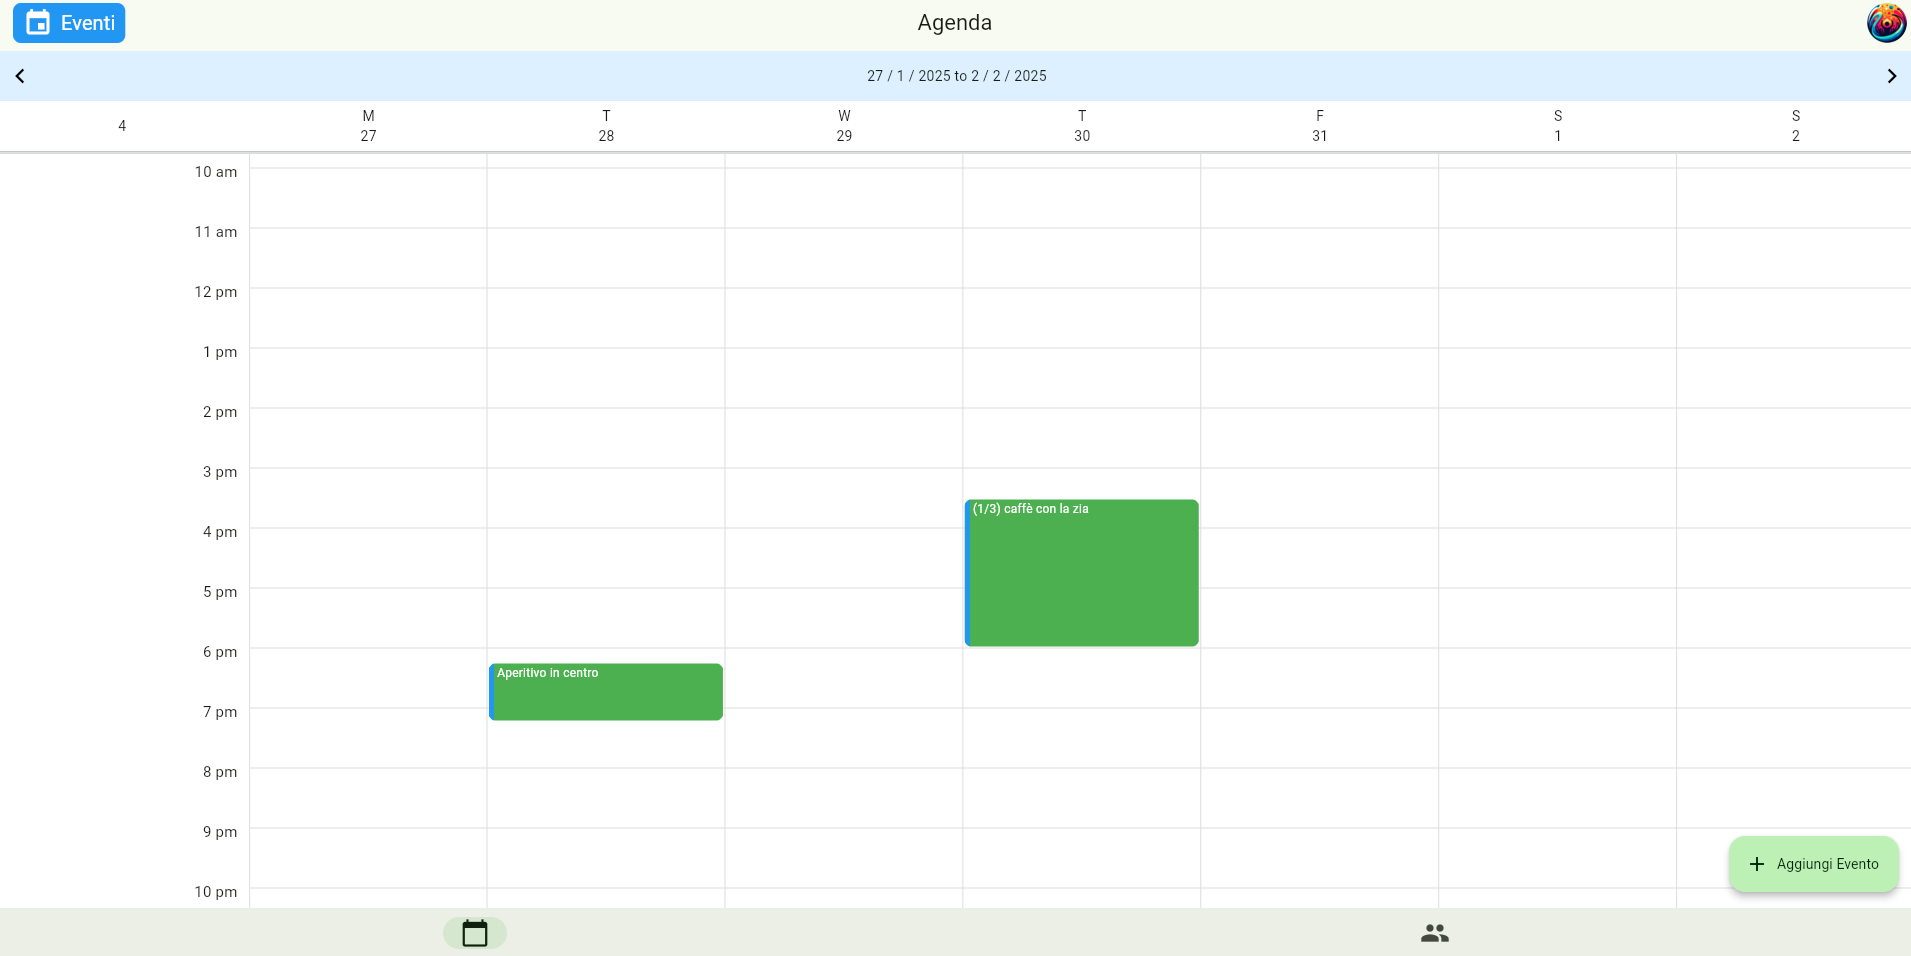
\includegraphics[width=\textwidth]{ProgettoVistaConfermati.png}
    \caption{Eventi confermati}
\end{figure}
\begin{figure}[h!]
    \centering
    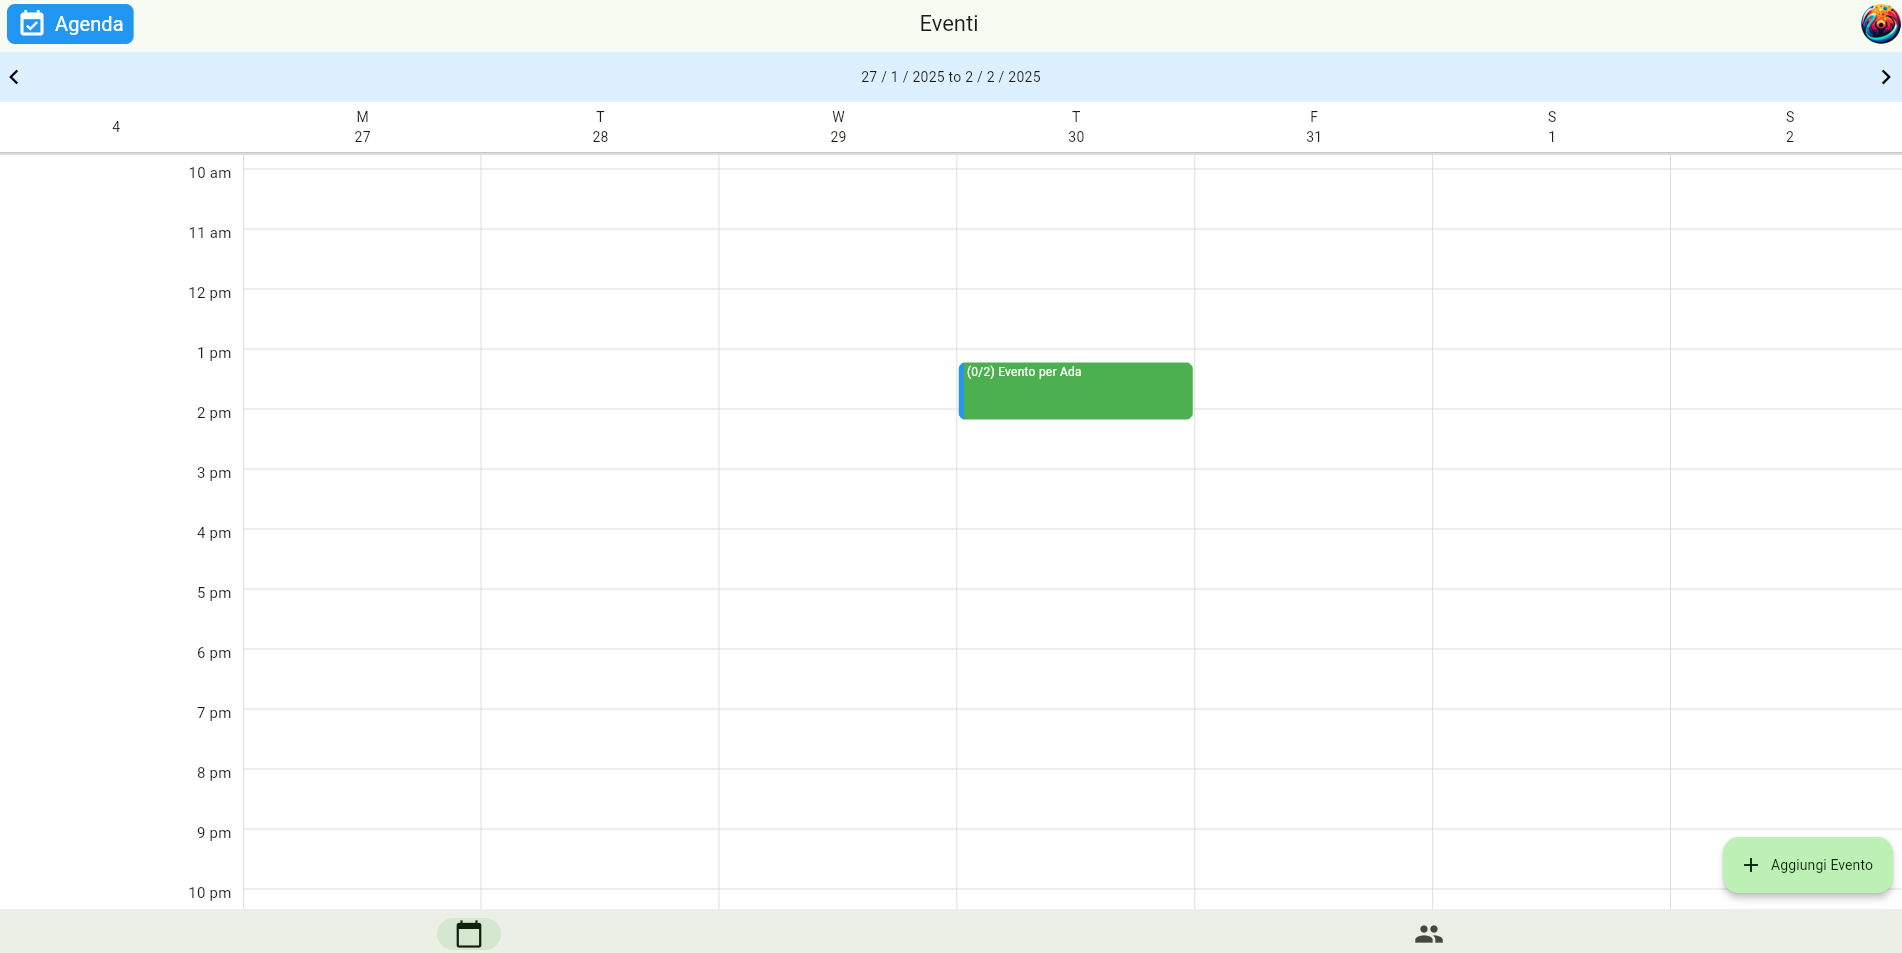
\includegraphics[width=\textwidth]{ProgettoVistaProposti.png}
    \caption{Eventi proposti}
\end{figure}
\begin{figure}[h!]
    \centering
    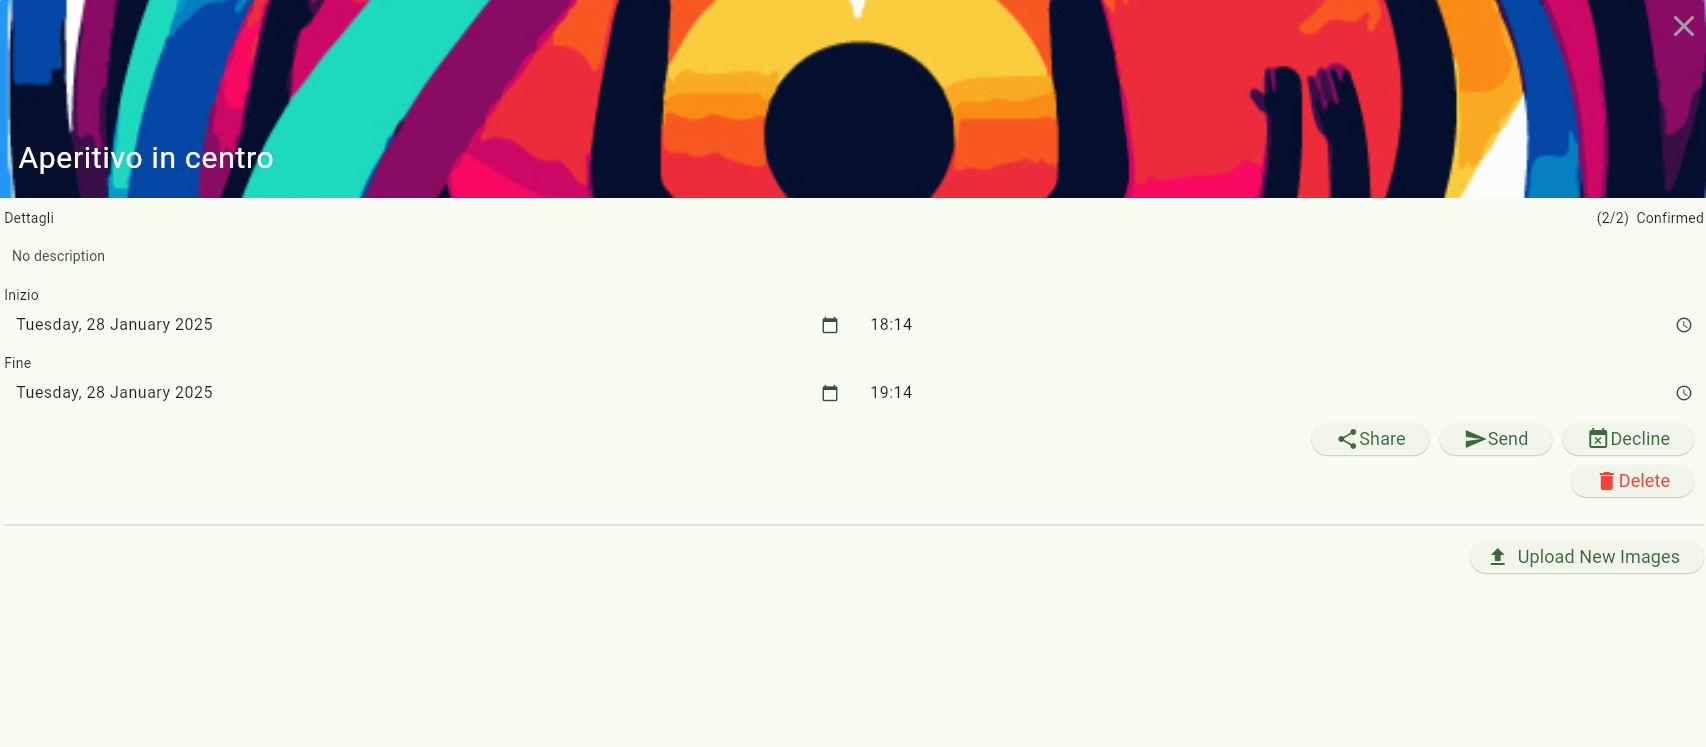
\includegraphics[width=\textwidth]{ProgettoVistaEvento.png}
    \caption{Dettaglio evento}
\end{figure}
\clearpage

\textbf{Diagramma di dettaglio: InterfacciaUtente - Gruppi}
\begin{figure}[h!]
    \begin{center}
        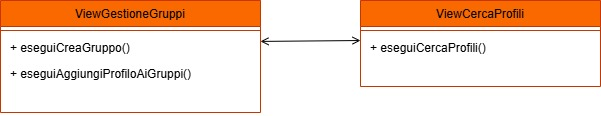
\includegraphics[width=0.9\textwidth]{ProgettoViewGruppi.jpg}
    \end{center}
\end{figure}
\begin{figure}[h!]
    \centering
    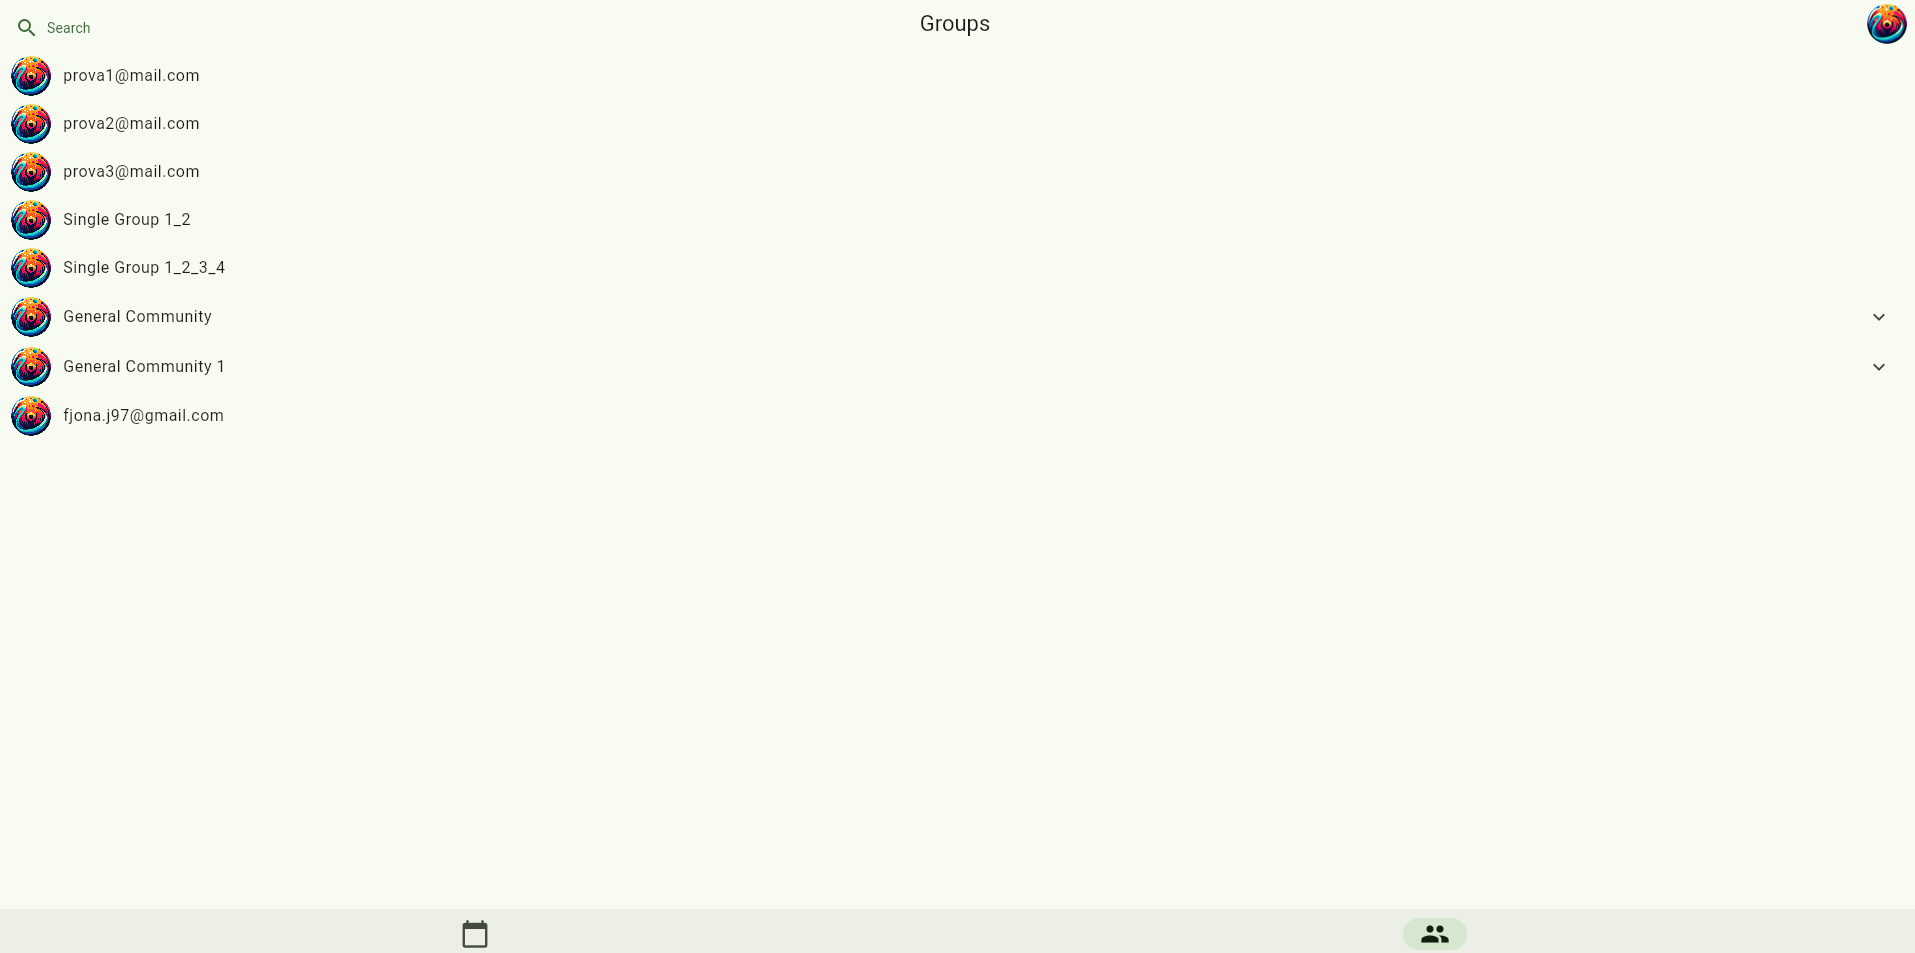
\includegraphics[width=\textwidth]{ProgettoVistaGruppi.png}
    \caption{Gruppi}
\end{figure}
\begin{figure}[h!]
    \centering
    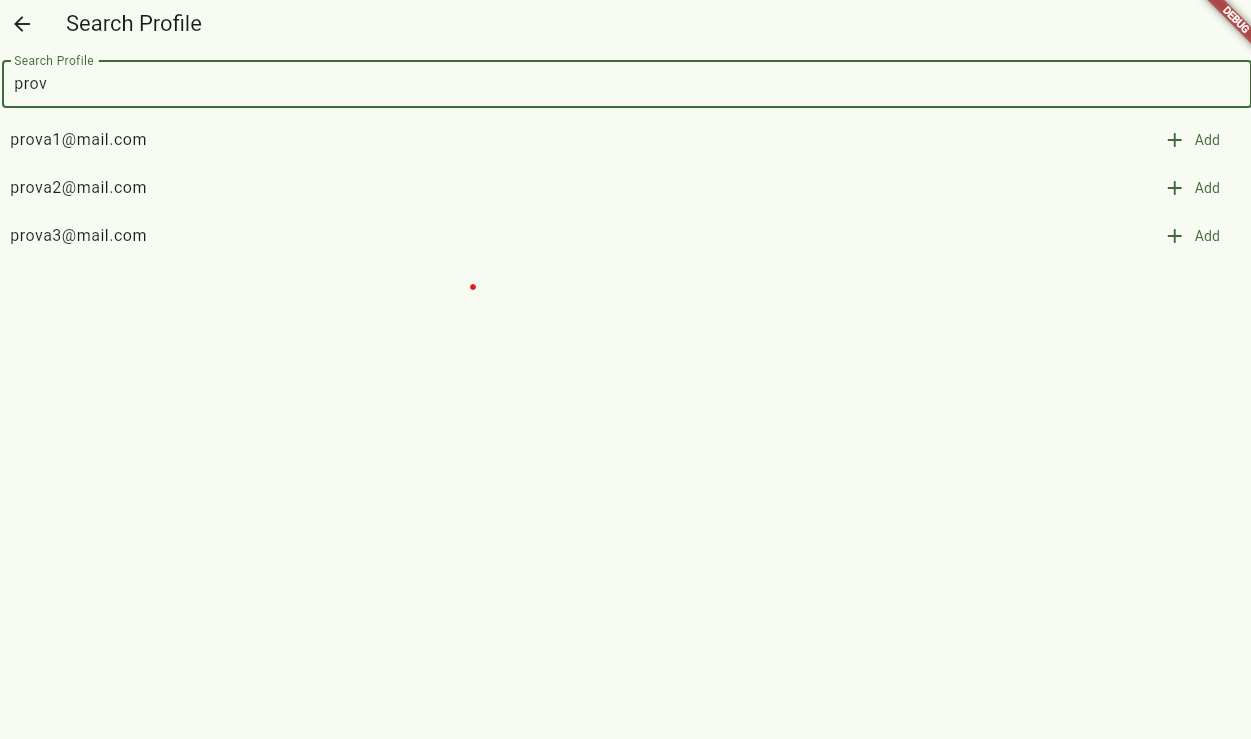
\includegraphics[width=\textwidth]{ProgettoVistaCercaProfili.png}
    \caption{Cerca profili}
\end{figure}
\clearpage

\textbf{Diagramma di dettaglio: InterfacciaUtente - Profili}
\begin{figure}[h!]
    \begin{center}
        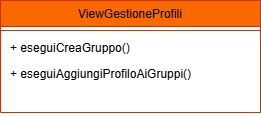
\includegraphics[width=0.6\textwidth]{ProgettoViewProfili.jpg}
    \end{center}
\end{figure}

\begin{figure}[h!]
    \centering
    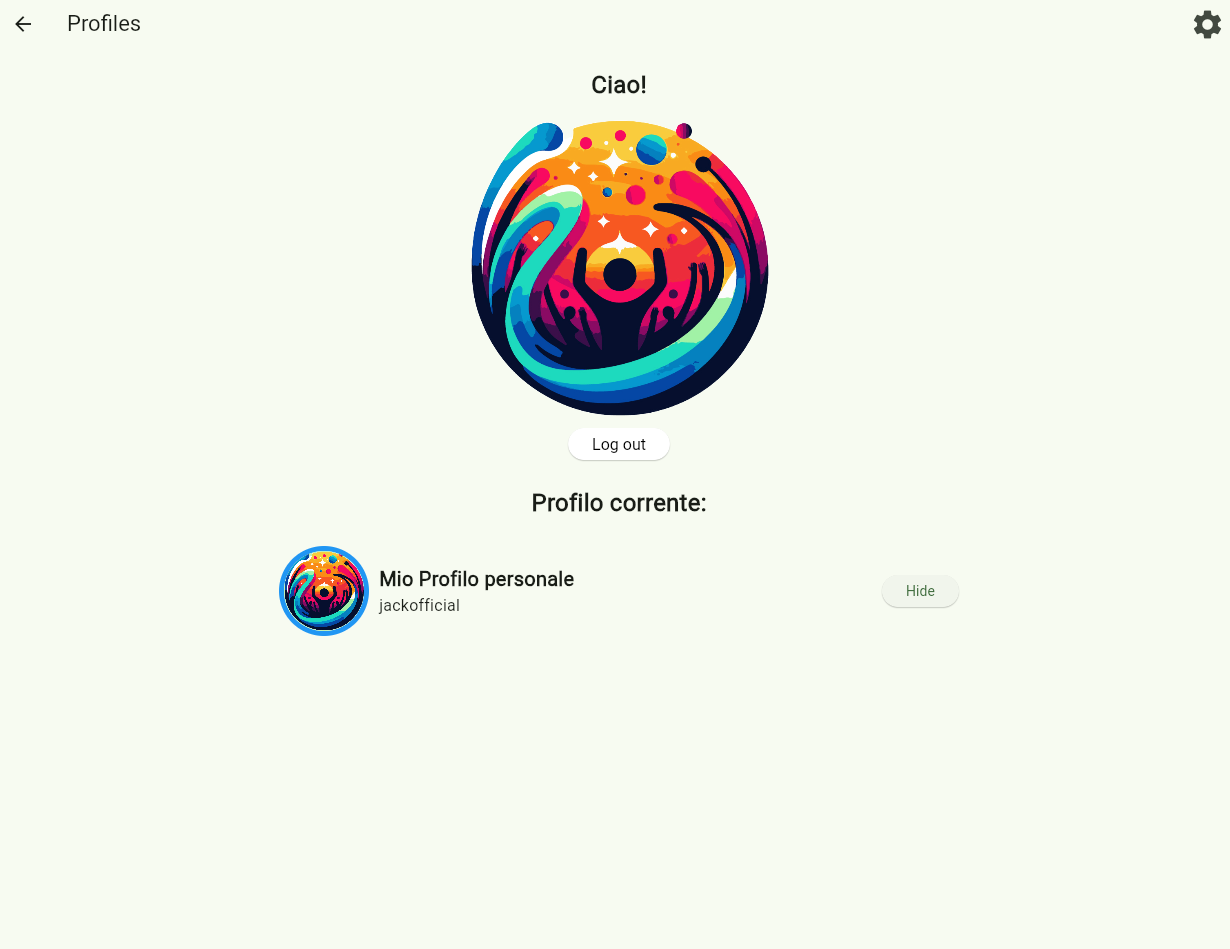
\includegraphics[width=\textwidth]{ProgettoVistaProfili.png}
    \caption{Profili collegati}
\end{figure}

\newpage

\textbf{Diagramma di dettaglio: InterfacciaGestioneAccesso}

\begin{figure}[h!]
    \begin{center}
        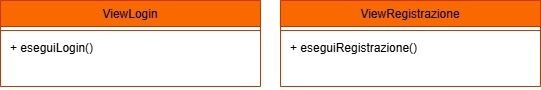
\includegraphics[width=0.9\textwidth]{ProgettoViewGestioneAccesso.jpg}
    \end{center}
\end{figure}

\begin{figure}[h!]
    \centering
    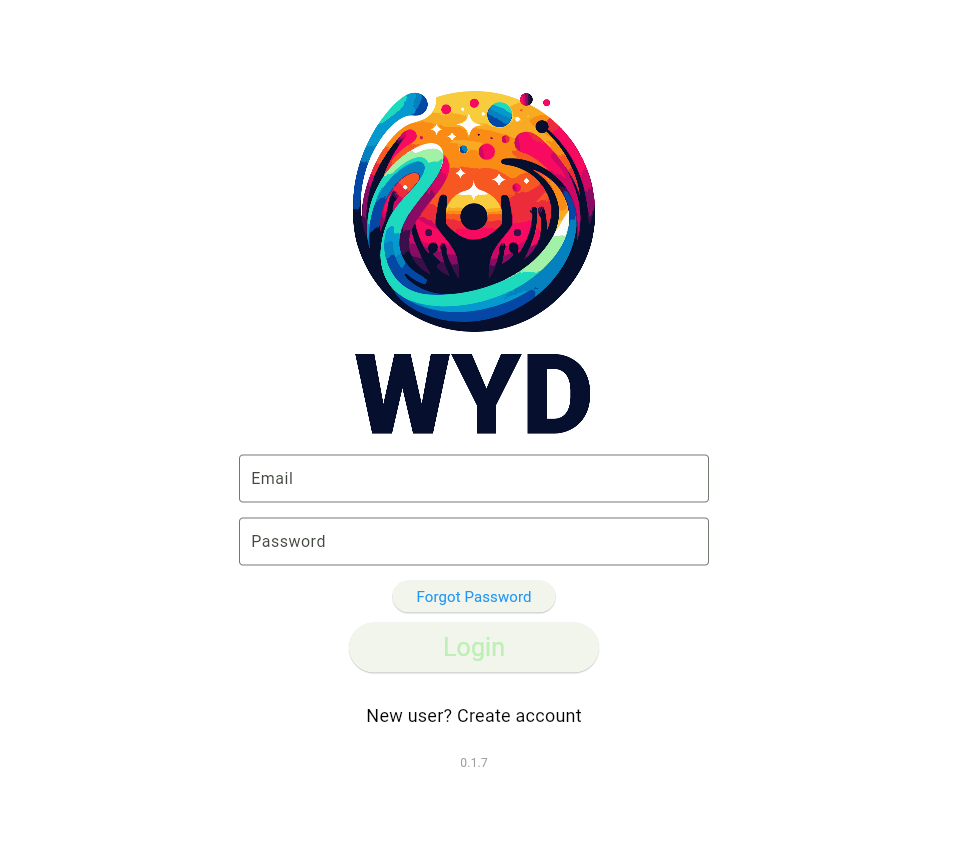
\includegraphics[width=\textwidth]{ProgettoVistaLogin.png}
    \caption{Login}
\end{figure}
\begin{figure}[h!]
    \centering
    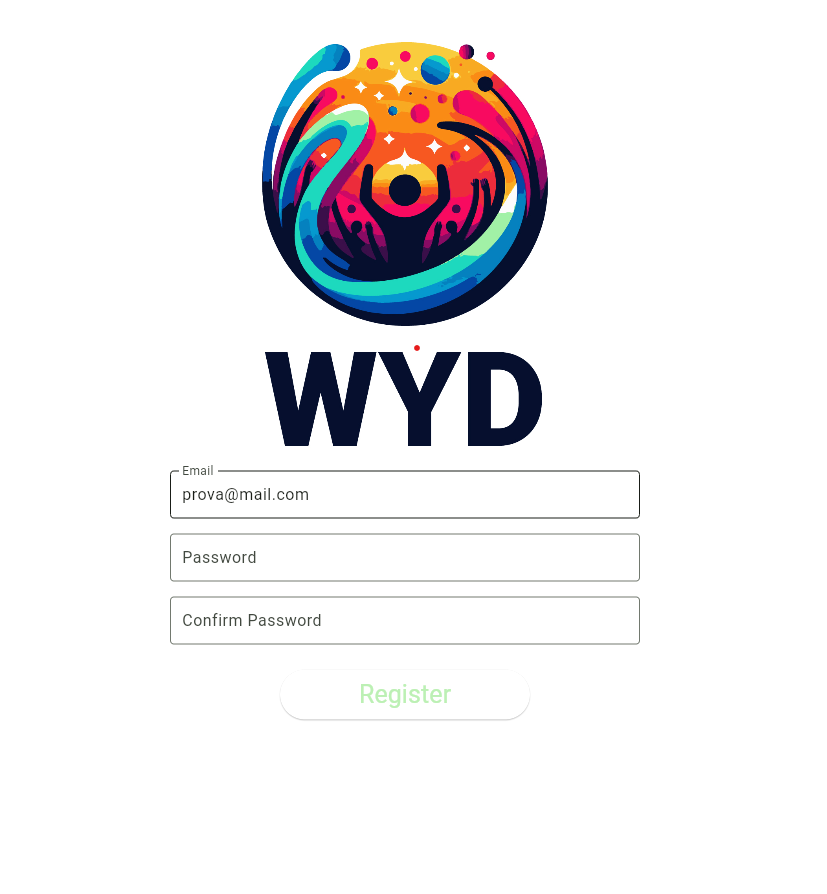
\includegraphics[width=\textwidth]{ProgettoVistaRegistrazione.png}
    \caption{Registrazione}
\end{figure}
 
\clearpage

\subsubsection{Interazione}

Si riportano di seguito i vari diagrammi di sequenza, aggiornati rispetto a quelli visti in fase di analisi.\\
TODO aggiungere GestioneAggiornamentiController
\vspace{3em}

\textbf{Diagramma di Sequenza: Registrazione}
\begin{figure}[h!]
    \centering
    \rotatebox{90}{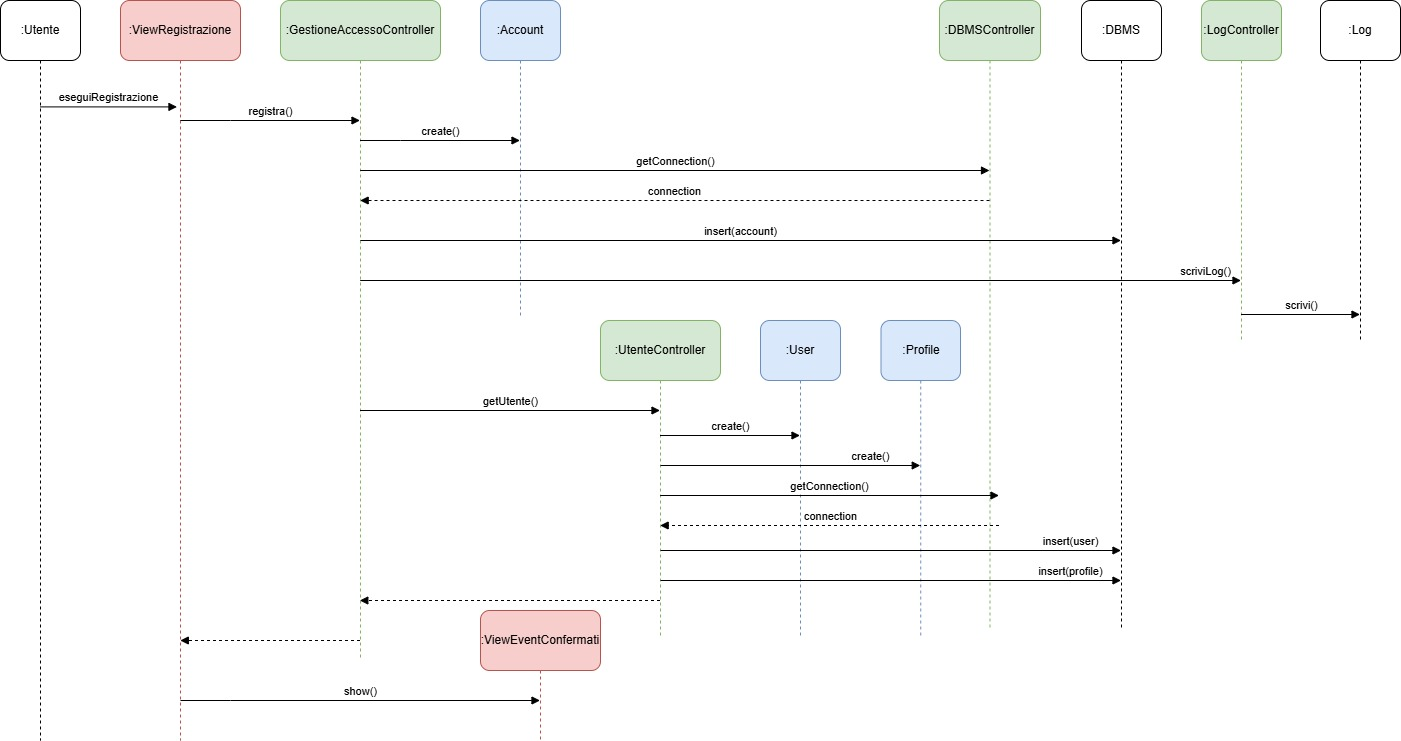
\includegraphics[width=\textwidth]{PIRegistrazione.jpg}}
\end{figure}
\clearpage
\textbf{Diagramma di Sequenza: Visualizza Eventi Confermati}
\begin{figure}[h!]
    \centering
    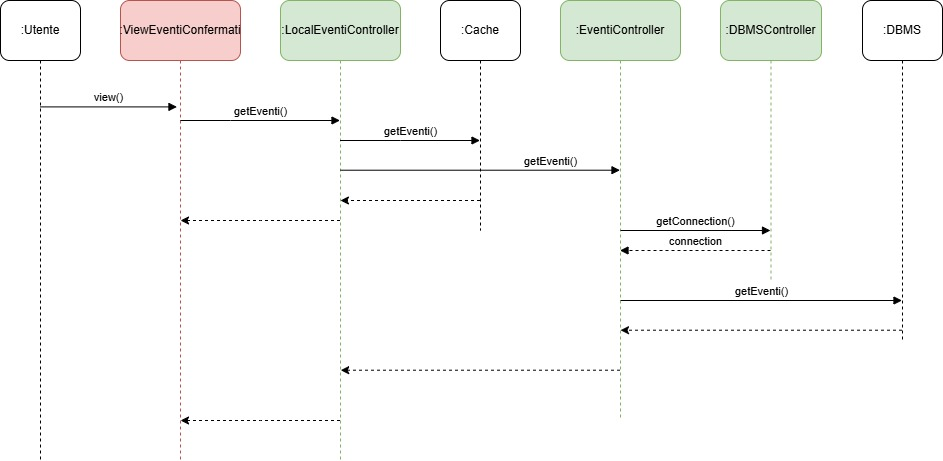
\includegraphics[width=\textwidth]{PIVisualizzaEventiConfermati.jpg}
\end{figure}\\
\textbf{Diagramma di Sequenza: Visualizza Evento}
\begin{figure}[h!]
    \centering
    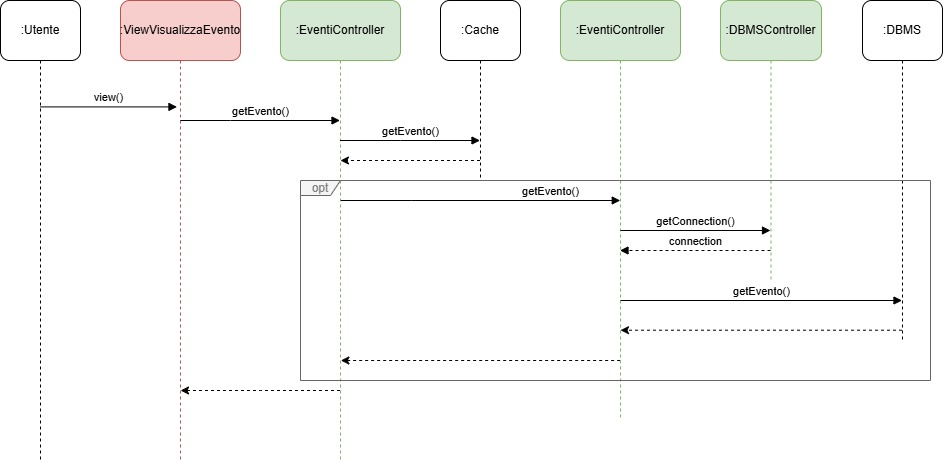
\includegraphics[width=\textwidth]{PIVisualizzaEvento.jpg}
\end{figure}
\clearpage
\textbf{Diagramma di Sequenza: Crea Evento}
\begin{figure}[h!]
    \centering
    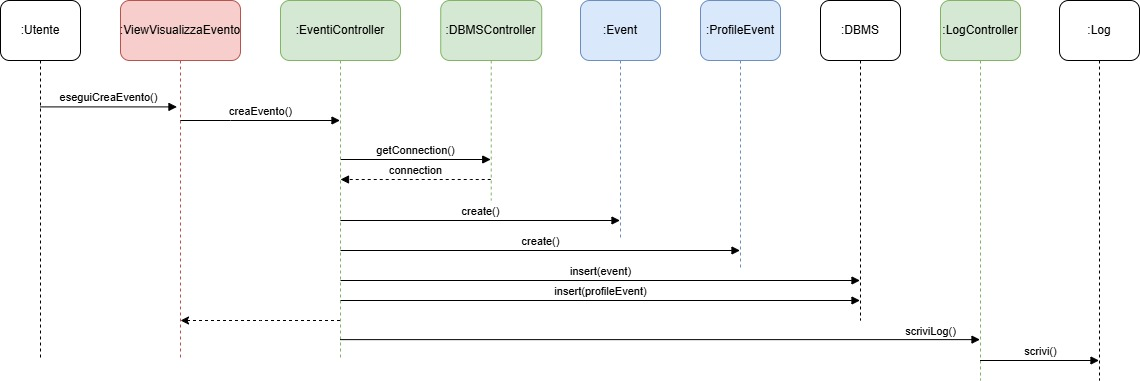
\includegraphics[width=\textwidth]{PICreaEvento.jpg}
\end{figure}\\
\textbf{Diagramma di Sequenza: Modifica Evento}
\begin{figure}[h!]
    \centering
    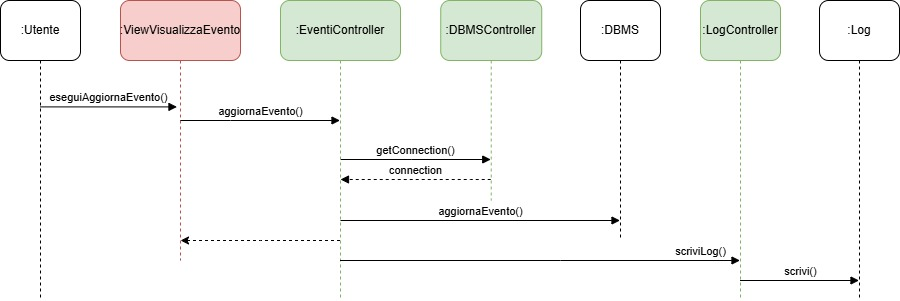
\includegraphics[width=\textwidth]{PIModificaEvento.jpg}
\end{figure}
\clearpage
\textbf{Diagramma di Sequenza: Conferma Evento}
\begin{figure}[h!]
    \centering
    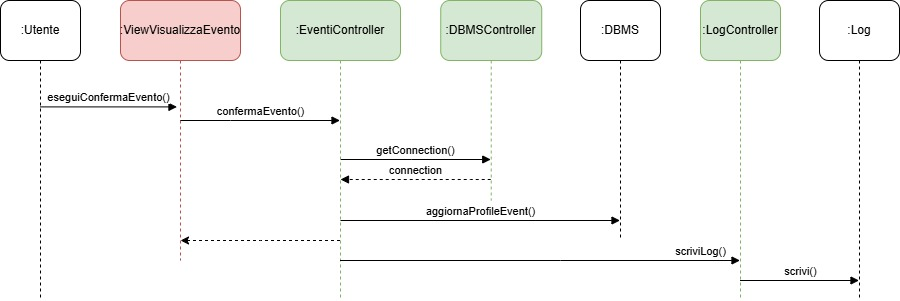
\includegraphics[width=\textwidth]{PIConfermaEvento.jpg}
\end{figure}
\clearpage
\textbf{Diagramma di Sequenza: Conferma Immagini}
\begin{figure}[h!]
    \centering
    \rotatebox{90}{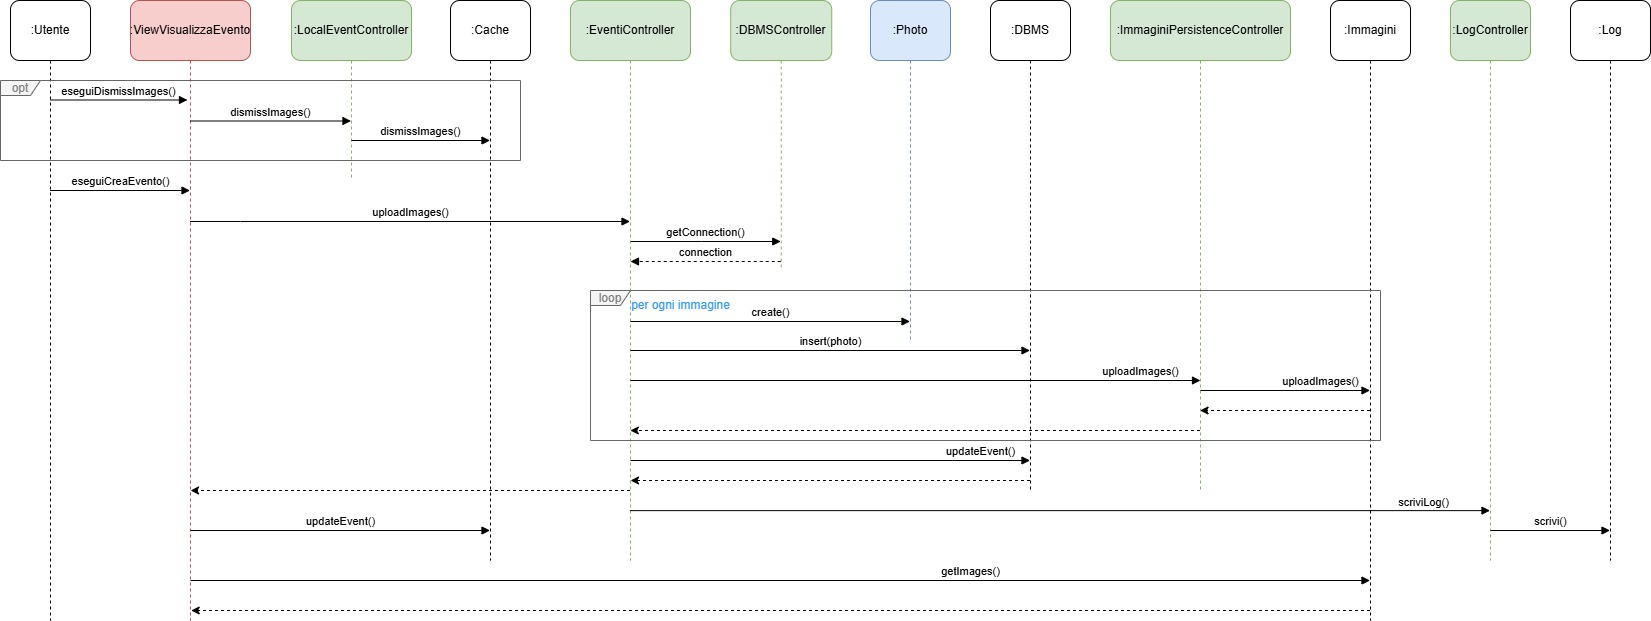
\includegraphics[width=\textwidth]{PIConfermaImmagini.jpg}}
\end{figure}
\clearpage

\textbf{Diagramma di Sequenza: condividi Evento ai Gruppi}
TODO\\
\textbf{Diagramma di Sequenza: Cerca profili}
TODO\\
\textbf{Diagramma di Sequenza: aggiorna}
TODO

\clearpage

\subsection{Progettazione della persistenza}

\subsubsection*{Diagramma E-R}

\begin{figure}[h!]
    \begin{center}
        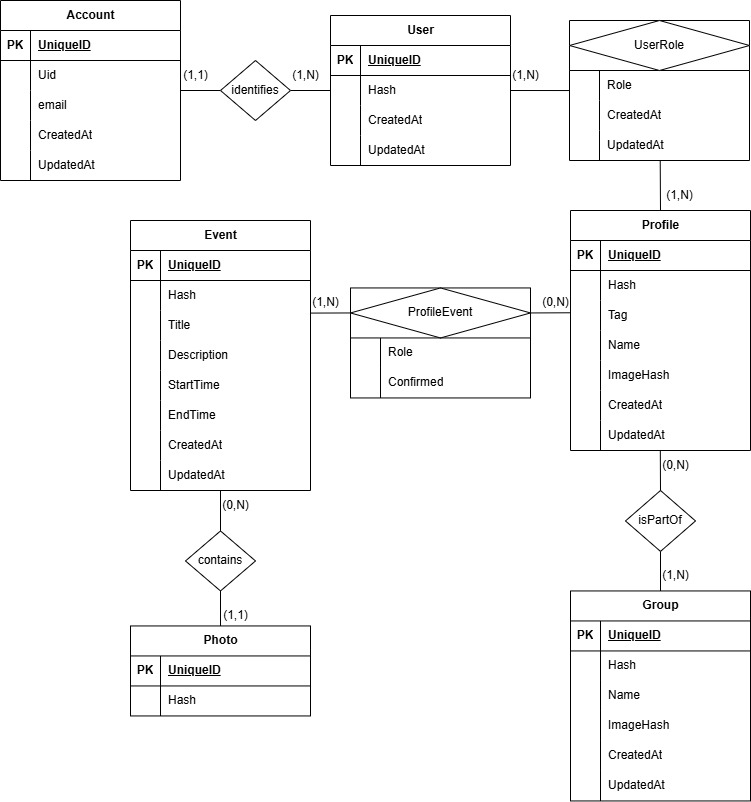
\includegraphics[scale=0.545]{ProgettoDiagrammaER.jpg}
    \end{center}
\end{figure}

Come si può notare, il diagramma E-R della persistenza segue precisamente la struttura del modello del dominio mostrato precedentemente.
La differenza sta nelle associazioni, che presumibilmente in fase di progettazione logica ed implementazione del database verranno concretizzate in classi di associazione,
si avranno quindi due tabelle ulteriori (\texttt{ProfileEvent} e \texttt{UserRole}) per modellare le associazioni.

\subsubsection{Formato dei file di log}

Il formato del file di log su cui il sistema terrà traccia delle operazioni
sarà il seguente:\\

Esempio: File \texttt{/var/log/wyd.log}\\

\texttt{\$ Data - Ora - Operazione - Descrizione - ID utente}\\
\textbf{Nota}: l'ID utente è l'identificativo dell'esecutore di tale operazione.
\newpage

%\subsection{Progettazione del collaudo}

%\vspace{2em}

%\subsection{Progettazione per il deployment}

%\newpage

\subsection{Deployment}

\subsubsection{Artefatti}

\begin{figure}[h!]
    \begin{center}
        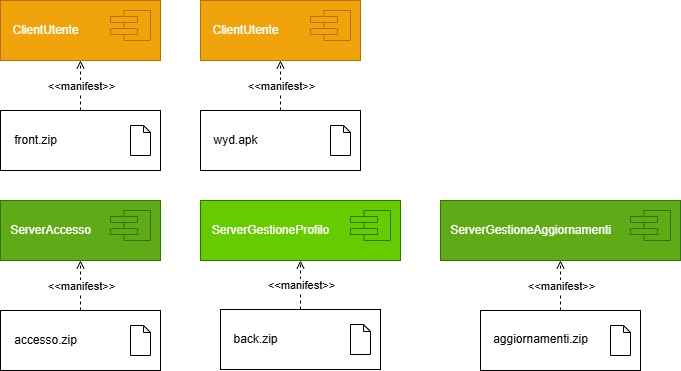
\includegraphics[width=\textwidth]{ProgettoDeploymentArtefatti.jpg}
    \end{center}
\end{figure}
\newpage
\subsubsection{Deployment Type-Level}

\begin{figure}[h!]
    \begin{center}
        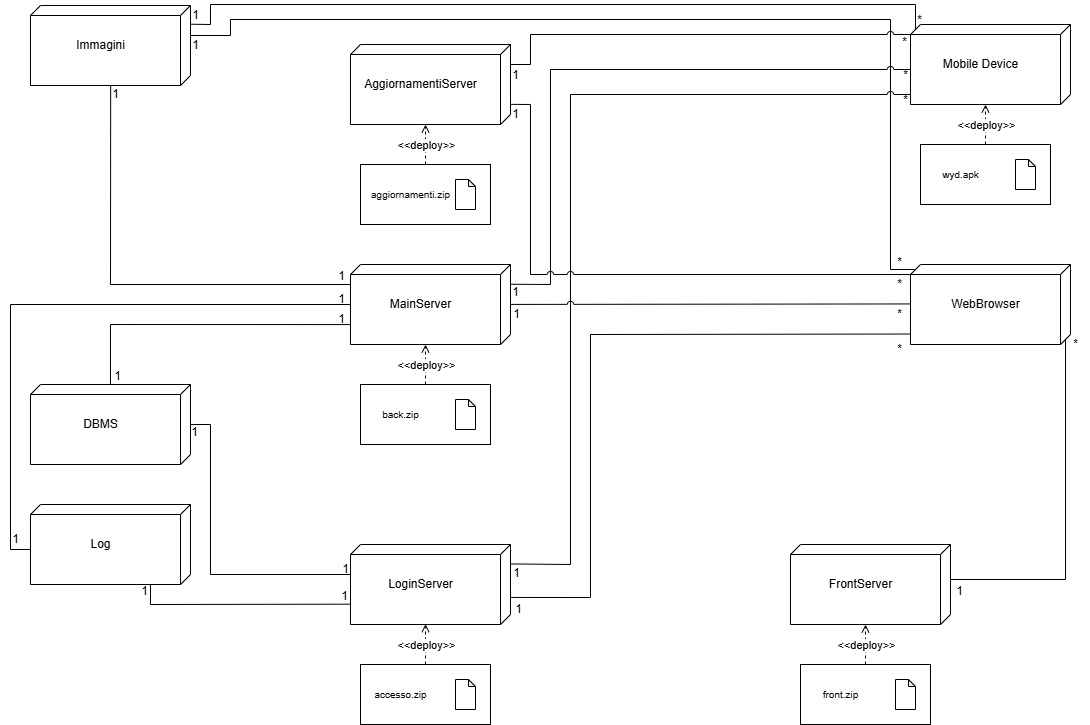
\includegraphics[width=\textwidth]{ProgettoDeploymentTypeLevel.jpg}
    \end{center}
\end{figure}

\end{document}
